
%TODO: Find out what's different about ns-proposal used in reliability proposal
% \documentclass[letterpaper,10pt]{article}
%% \documentclass[10pt,onecolumn]{article}
\documentclass[10pt,onecolumn]{ns-article}
% \newcommand{\mydriver}{pdflatex}
% \documentclass[12pt,\mydriver]{thesis-2}
%% \usepackage[letterpaper, margin=1.25in]{geometry} % For giving to neil


\PassOptionsToPackage{hyphens}{url}
\usepackage[hyphens]{url}
\usepackage{hyperref}
\hypersetup{breaklinks=true}
\urlstyle{same}
\usepackage{balance}

% TODO: I seem to have used most of these from the reliability
% proposal. Find out what the role of each command is.
\usepackage{ifpdf,floatrow} 

% nspring 10.35pt palatino
\renewcommand*{\rmdefault}{ppl} % Roman default
\usepackage{fix-cm}
% \renewcommand{\normalsize}{\fontsize{10.35pt}{12.5pt}\selectfont}
% \renewcommand{\normalsize}{\fontsize{10pt}{12.5pt}\selectfont}
% endspring

%% ns - replacement for times that lacks stupidity.
% \usepackage{mathptmx}
% \usepackage[scaled=.90]{helvet}
% \usepackage{courier}
% 
% \usepackage[override]{cmtt} % make tt font tighter / less ugly

% \usepackage{makeidx}  % allows for indexgeneration

\usepackage[square,comma,numbers,sort&compress]{natbib}

\usepackage{titlesec}
   \titleformat{\chapter}
      {\normalfont\large}{Chapter \thechapter:}{1em}{}

\usepackage{color}
\usepackage[table]{xcolor}
\definecolor{orange}{RGB}{255,127,0}
\newcommand{\rama}[1]{{\color{red}[\todo{rama: #1}]}}
\newcommand{\ns}[1]{{\color{green}[ns: #1]}}
\newcommand{\etal}{et~al.\xspace}
\providecommand{\ie}{\emph{i.e.,} }
\providecommand{\eg}{\emph{e.g.,} }
\providecommand{\cf}{\emph{cf.,} }
\providecommand{\vs}{\emph{vs.} }
\providecommand{\etc}{\emph{etc.}}   
\providecommand{\ione}{\emph{(i)} }
\providecommand{\itwo}{\emph{(ii)} }
\providecommand{\ithree}{\emph{(iii)} }
\providecommand{\ifour}{\emph{(iv)} }
\providecommand{\ifive}{\emph{(v)} }

% \newcommand{\ignore}[1]{}

% Rk: The following commands came from the NSF reliability proposal
% \setlength{\textwidth}{6.5in}
% \setlength{\textheight}{9in}
% \setlength{\topmargin}{0in}
% \setlength{\headheight}{0in}
% \setlength\columnsep{.30in}
% \setlength{\headsep}{0in}
% \setlength{\oddsidemargin}{0pt}
% \setlength{\evensidemargin}{0pt}

% Rk: The following commands are from mainthesis.tex from UMD's
% official style guide. Revisit and fix to get tables.
% \newcommand{\tbsp}{\rule{0pt}{18pt}} %used to get a vertical distance after \hline
% \renewcommand{\baselinestretch}{2}
% \setlength{\textwidth}{5.9in}
% \setlength{\textheight}{9in}
% \setlength{\topmargin}{-.50in}
% %\setlength{\topmargin}{0in}    %use this setting if the printer makes the the top margin 1/2 inch instead of 1 inch
% \setlength{\oddsidemargin}{.55in}
% \setlength{\parindent}{.4in}
% \pagestyle{empty}

\setlength{\textfloatsep}{.1in plus 0.05in}
\setlength{\itemsep}{-10pt}


\usepackage{enumitem}
\setlist[itemize]{leftmargin=*}
% \usepackage{slashbox}
\usepackage{graphicx}
\usepackage{amsmath,amssymb}
\usepackage{verbatimbox}
\usepackage{boxedminipage}
\usepackage{multirow}
% \usepackage{subfigure}
\usepackage[labelformat=simple]{subcaption}
% \usepackage{subfig}
\usepackage{xspace}
\usepackage[]{pdfpages}

\usepackage[utf8x]{inputenc}
\usepackage{ucs}

% \newcounter{FileStack}
% \let\OrigInput\input
% \newcommand{\ninput}[1]{%
%   \stepcounter{FileStack}
%   \expandafter\let
%   \csname NameStack\theFileStack\endcsname
%   \ThisFile
%   \def\ThisFile{#1}%
%   \OrigInput{#1}%
%   \expandafter\let\expandafter
%   \ThisFile
%   \csname NameStack\theFileStack\endcsname
%   \addtocounter{FileStack}{-1}%
% }

%boxed,vlined,,linesnumbered,commentsnumbered
\usepackage[vlined]{algorithm2e}
\providecommand{\SetAlgoLined}{\SetLine}
\providecommand{\DontPrintSemicolon}{\dontprintsemicolon}





\newcommand{\planetlab}{PlanetLab\xspace}

% \renewcommand\thesubfigure{(\alph{subfigure})}

%\usepackage{algorithm}s}
\title{Analyzing Internet reliability remotely for
  individual users with probing-based techniques}
% \title{Thesis Proposal: Remote probing-based outage detection for
%   individual IP addresses}

\author{Ramakrishna Padmanabhan}

\begin{document}

% Define table specific commands
\newcommand{\bb}{~~~~~}
\newcommand{\hdr}[1]{\multicolumn{1}{c}{\textbf{#1}}}
% define ``struts'', as suggested by Claudio Beccari in
%    a piece in TeX and TUG News, Vol. 2, 1993.
\newcommand\Tstrut{\rule{0pt}{2.2ex}}         % = `top' strut
\newcommand\Bstrut{\rule[-0.9ex]{0pt}{0pt}}   % = `bottom' strut

\maketitle


\begin{abstract}

% We use the Internet without know that the Internet is actually super reliable. It's based more upon: hey, the Internet seems reliable. 

% The Internet is used today for communication

% Detection of Internet outages, which are potentially rare events, demands broad and longitudinal measurements of users' Internet connections.
% Internet reliability is increasingly important as the applications we use increasingly depend upon the Internet.
% Internet reliability is increasingly important as a variety of services that we use migrate to the Internet.
% Internet reliability is increasingly important as the applications that we depend upon migrate to the Internet.
Internet reliability is increasingly important as a variety of services that we use migrate to the Internet. Yet, we lack authoritative measures of last-mile Internet reliability. The first step towards measuring last-mile reliability is to detect Internet outage events experienced by users. Since Internet outages are rare events, detecting them requires broad and longitudinal measurements; however, such measurements of Internet reliability at the individual user level are challenging to obtain accurately and at scale. The second step is to use detected outages to reason about Internet reliability across different dimensions such as ISPs, media-types, and geographical areas.

Probing-based remote outage detection techniques can scale but their accuracy is questionable. These techniques detect Internet outages across time as well as across the IPv4 address space by sending active probes, such as pings and traceroutes, to users' IP addresses and use probe responses to infer Internet connectivity. However, they can infer false outages since their foundational assumption can sometimes be invalid: that the lack of response to an active probe is indicative of failure. I illustrate two potential scenarios where this assumption is invalid. In the first scenario, responses are delayed beyond the prober's timeout, leading these techniques to infer packet-loss instead of delay. In the second scenario, these techniques can falsely infer packet-loss when the address they are probing gets dynamically reassigned. I examine how commonly delayed responses and dynamic reassignment occur across ISPs to quantify the inaccuracy of these techniques. 

Next, I demonstrate how detected outages can be used to perform meaningful assessments of Internet reliability. One aspect of Internet reliability is the study of how an external factor (like the occurence of thunderstorms) affects Internet connectivity; I show how to study the effect of such a factor upon the reliability of a group of addresses by studying the \emph{inflation} in outage rate for that group during its presence. Measuring the inflation in outage rate mitigates the effects of false outages. I also develop and evaluate an approach to segregate outages into categories that suggest their cause. Outages could result from a variety of causes, such as power outages, voluntary shutdown of users' home Internet equipment, network outages due to an ISP's infrastructure failure etc. When assessing the reliability of a particular ISP, we would ideally consider only the subset of outages that affect solely that ISP. I propose a technique to segregate outages by detecting simultaneous outages of ``related'' groups of addresses (addresses may be related by geography, ISP, or network topology). Simultaneous outages can serve as evidence that a detected outage affected multiple users in a particular ISP.

Implementing these proposed techniques will help achieve comprehensive measurements of Internet reliability that can be used to identify vulnerable networks and their challenges, inform which enhancements can help networks improve reliability, and evaluate the efficacy of deployed enhancements over time.

% comprehensive datasets of Internet reliability that can aid in improving reliability by targeting problem regions or adapting strategies that have proven to be successful
\end{abstract}

\newpage


% \section{Preliminaries}

\section{Introduction}


% With online accessibility of
% devices ranging from temperature control systems to baby monitors in
% this Internet of Things era, our dependence upon the Internet for
% increasingly many facets of our daily lives only continues to
% rise.

% With the ability to access a
% variety of devices online in this Internet of Things era, ranging from
% temperature control systems to baby monitors, our dependence upon the
% Internet for increasingly many facets of our daily lives only
% continues to rise. 

% As the range of Internet services that we rely upon increases, so does our reliance upon
% the Internet. 

% Talk more about how important the Internet is?

Residential Internet reliability is increasingly important as a variety of
services that we use migrate to the Internet. Internet users today can
communicate with each other, perform financial transactions, plan
their travel, and even obtain critical services such as health
monitoring~\cite{ideal-life, remote-health-elderly} and emergency
services~\cite{emergency-voip-voipfone, emergency-voip-fcc} from their
homes. Our dependence upon the Internet will rise further as more of
our home devices become connected in this Internet of Things
era. Consequently, continuous availability of the Internet and
resilience is vital, and the reliability of the Internet is of
interest to stakeholders across the board, from government regulators and
Internet Service Providers, to users.

% TODO: How do I connect the next sentence neatly to the previous
% paragraphs? Especially when the previous paragraphs will go on to
% talk about all the interested parties at length.

% TODO: Look into billionts for citations about regulator interest.

Broad and longitudinal
measurements of users' Internet reliability in different circumstances
can identify vulnerable networks and their challenges, can inform
which enhancements can help these networks improve reliability, and
can evaluate the efficacy of deployed enhancements.

% Measuring
% Internet reliability at the individual user level will therefore prove invaluable in assessing
% the current state of Internet connectivity and in developing future
% enhancements.

% By detecting outage events and their duration, we
% can reason about a particular user's Internet reliability and compare
% it to other users' reliability across geography, ISPs, and
% media-types.

% Talk about how Internet reliability is difficult and who is
% interested. FCC. Even ISPs (Cite the "Nevermind" paper by Nick
% Duffield which claims that ISPs are typically reactive and wait for
% customers to call). Common users.

Yet, we lack authoritative measures of last-mile Internet reliability. The first step towards measuring users' Internet
reliability is to detect \emph{Internet outages}---events that prevent
users from communicating over the Internet. Since we expect outage
events to be rare, detecting them requires broad and longitudinal
measurements of individual users. However, such measurements of
Internet reliability at the individual user level are challenging to
obtain accurately and at scale. The next step towards measuring users'
reliability is to segregate detected outages into categories
that suggest their cause. Once outages are categorized in this
manner, we can estimate the reliability of an ISP by considering the
subset of outages that affected solely that ISP.

Existing techniques that measure individual-user-level outages can be
grouped into on-premises outage detection techniques and remote probing-based
outage detection techinques. On-premises techniques, such as
RIPE Atlas~\cite{atlas}, SamKnows~\cite{samknows}, and
BISmark~\cite{bismark-main-bib}, measure diverse aspects of
users' Internet connections, but
measure relatively few users. These techniques 
deploy dedicated hardware at user premises that continuously conduct ping,
traceroute, DNS measurements etc.; some of these
measurements can be used to infer Internet connectivity problems. Whereas hardware
based techniques have fundamental scaling difficulties owing to
manufacturing and deployment costs, hundreds of millions of
IP addresses respond to active probes~\cite{timeouts}. Since many
residences have at least one device with a public IP address ~\cite{cgn-imc16}
(typically the home router), these IP addresses can be probed
remotely, from 
vantage points that we control, to measure their connectivity. Thunderping~\cite{pingin} and Trinocular~\cite{trinocular} adopt this
approach to outage detection, taking a
complementary approach to on-premises techniques: they focus upon
measuring only connectivity but do so for many users. Since these
techniques can send probes remotely from servers under their control, without requiring any user
involvement, they are able to detect outages across time
as well as across the IPv4 address space.
% However, existing techniques do
% not study latency and therefore do not identify performance
% degradation resulting from high delay.
However, probing-based remote outage detection techniques can
make false inferences about outages when some scenarios
occur~\cite{timeouts, addrchange-reasons}. Further, existing
techniques have not 
attempted to categorize detected outages by their likely cause.
% However, measuring residential
% outages is challenging because of the scale: there are millions of
% residential links to measure. 
% Second, users can voluntarily power
% down their home Internet equipment and it is challenging to
% distinguish between voluntary user shutdowns and an outage at the last-mile link.
 
% ; even multihomed last mile links for business connectivity
% often share the same upstream hardware, representing a single point of 
% failure~\cite{twcable-business-web}. 
% Last-mile links lack the redundancy of the Internet's core;
% thus an outage of the last-mile link is likely to cut off users'
% Internet connectivity altogether.

% The second challenge is that it can be hard to distinguish
% between an outage at the last-mile link and voluntary user shutdowns
% of their Internet connections.
% We do not have a good understanding of the reliabity of Internet
% connectivity for end-users. Understanding the reliability of Internet
% connectivity for end-users requires understanding the reliability of
% the \emph{last mile link} connecting an end-user to the Internet. This
% is because the core of the Internet is designed to be redundant but
% last mile links typically are not.
%TODO: Perhaps borrow sentence from enduser.tex about business last-mile links.


% Thesis statement comments

% Older versions of thesis statement:
% \emph{For any end-host with a publicly assigned IP address that has the ability to respond to active probes, it is possible to remotely isolate accurately determine connectivity problems experienced by that end-host's last mile link.}
% \emph{For any end-host with an IP address that has the ability to
% respond to active probes, it is possible to remotely detect outages
% experienced by that end-host's last mile link.}

% Bobby's comments: Send traceroutes, but also to related addresses. What happens when all addresses change en-masse? Can we somehow identify such instances?
% Neil suggested that I should replace end-host with 'Internet accessible device'. Can I assert that a device with a public IP address is by definition Internet accessible.
% \emph{It is possible to remotely and accurately detect outages experienced by any device with a public IP address that typically responds to active probes.}

% Come up with definition of accuracy of outages.

% and use it to compare reliability across ISPs, media-types and
% geographical areas

I argue in this thesis that 
\emph{It is possible to remotely and accurately detect substantial outages
  experienced by any device with a stable public IP address that typically
  responds to active probes and use these outages to compare
  reliability across ISPs, media-types and geographical areas.} To demonstrate the thesis, I make the following
initial contributions:

% TODO: 
% It is possible to remotely and accurately estimate the reliability of
% an ISP's customer's device so long as the device has
% a stable public IP address that typically
%   responds to active probes


In Section~\ref{sec:related}, I define terms in the thesis statement, place the problem of outage detection
at the individual user level in the context of related work, and describe the challenges
that probing-based remote outage detection techniques will need to address. These
techniques study outages by sending active probes (such as ping's echo
requests) and use probe responses to infer outages. They assume that a
response to an active probe indicates a working path to the probed
user device and that lack of response is indicative of failure. I
illustrate two scenarios where this assumption can be
invalid, leading to potentially false outage inferences.
 % I
% illustrate two potential scenarios where this assumption is
% invalid---when responses are delayed beyond the prober's timeout and
% when the probed address is dynamically reassigned. I also highlight why
% Internet outages voluntarily caused by the
% residential user need to be segregated.
% I also describe the challenge that remote probing-based techniques face
% in detecting outages specifically in the last-mile.

In Section~\ref{sec:timeouts}, I investigate the prevalence of delayed
probe responses due to early timeout. The
lack of response to an active probe isn't always indicative of loss;
for example, when
responses are delayed beyond the prober's timeout, the response
eventually arrives but the prober would never see the response because
it timed out too early. I report how commonly responses are delayed
beyond timeouts in
networks around the world and propose techniques to mitigate this
problem. 
% Decouple probe retransmission
% and loss. Possibly identify that only cellular guys have long delays?
% Also, this will ensure that we trigger retransmission upon high
% latency/loss and actually identify loss as loss and high latency as
% high latency.

In Section~\ref{sec:addr_change}, I investigate how dynamic addressing can
lead remote probing-based outage detection techniques to make false inferences about outages and techniques to
mitigate these false inferences. My approach to mitigating
these false inferences is rooted in building a model that characterizes
the probability that a dynamic address is reassigned at any point of time. I describe preliminary
work which shows the feasibility of building such a model and detail
proposed work to gather new datasets that can feed into the
model. I will ultimately use this model to find candidate stable Internet
addresses for probing.

In Section~\ref{sec:last_mile}, I discuss an approach to determine
which of the detected outages are consistent with the failure of an
ISP's operated equipment, and which outages can be attributed to other
causes such as power outages or users voluntarily shutting down their home
Internet equipment. My approach is to probe addresses that are related
to the address that is already being probed. I propose the use of multiple criteria
to find related addresses such as geography, ISP, and network
topology. I describe how we can then use simultaneous outages of these
related addresses (or the lack thereof) to categorize outages and
estimate Intrenet reliability along various dimensions.

% We show in this proposal that confounding factors can cause RODWAP
% techniques to sometimes
% infer false outages. 

% However, we argue that RODWAP techniques can
% be used for accurate outage detection by identifying and mitigating
% confounding factors. 
 % This has
% been the basis of existing active probe based techniques that detect
% loss, and thereby outage events, such as Thunderping~\cite{pingin} and
% Trinocular~\cite{quan2013trinocular}.

% In spite of , we argue that it is possible to remotely detect
% outages on the last mile link using active probes for any end-host
% with an IP address that responds to active probes.

% We investigate potential causes that
% would lead existing active probe based outage detection approaches to
% falsely infer loss and describe proposed work to mitigate detection of
% false loss in Section~\ref{sec:timeouts} and
% Section~\ref{sec:addr_change}. We also propose 

% We show in this proposal that probe-loss need not always be due to
% lossy links.


% \begin{itemize}
%   \item{\bf{False probe-loss inference due to early timeout:}} 
%     Traditionally, active probe based approaches time out probes after a few seconds. Responses that arrive after the timeout will be reported as lost. When this happens, existing techniques would confuse high delay with probe-loss.
%   \item{\bf{False probe-loss inference due to IP address change:}}
%     Consider an IP address that was previously responsive. If the host to whom that IP address was assigned changed its IP address as a result of dynamic addressing or mobility, and if the probed IP address is not reassigned to any host, then echo responses will cease to arrive and existing techniques would infer false probe-loss.
% \end{itemize}

% After analyzing causes of false probe-loss, we will investigate techniques to remove false probe-loss. Once we remove false probe-loss, we will be left with all instances of true probe-loss and probe-delays. This will give us the ability to identify that \emph{some} link on the path to the destination is experiencing connectivity problems. However, since we are specifically interested in identifying connectivity problems on the last-mile link we require another step. In this step, we will conduct TTL-limited probing from multiple vantage points to identify which link exhibits connectivity problems.




\chapter{Measuring Residential Internet
  Reliability: a Primer}

\label{cpt:bg}

In this chapter, I provide background and definitions related to the
thesis statement. Then I present related work in measuring Interne
outages in general, and residential Internet outages at the individual
user level in particular. I discuss probing-based techniques to detect
outages remotely in detail and illustrate scenarios where they could
make false inferences about outages. I also illustrate that measuring
Internet reliability using detected outages has nuances and show how
some classes of detected outages need to be treated differently,
depending upon the Internet reliability measure under consideration.

% In this dissertation, I focus
% upon how common outages are and therefore use the \emph{rate} at which
% outages occur. Another metric is the proportion of total measured time detected as outage events.


\section{Background and definitions}

Intuitively, a reliable Internet connection is one that works
continuously. In other words, it experiences no outages. 

Measuring Internet reliability, therefore, necessitates measuring
Internet outages and then using measured outages in a metric that
represents some property of outages. Depending upon the application,
the appropriate outage metric may vary.

The goal of this dissertation is to provide broad, longitudinal, and accurate measurements of
Internet reliability across ISPs, media-types, and geographic
locations in a variety of circumstances. Such measurements can help
users choose from their available Internet options and can inform ISPs
about potential problems in their networks. To achieve this goal, I
propose the following thesis and define terms in the thesis as follows:



\emph{It is possible to remotely and accurately detect substantial outages
  experienced by any device with a stable public IP address that typically
  responds to active probes and use these outages to compare
  reliability across ISPs, media-types and geographical areas.}


\begin{itemize}

\item {\emph{Device with a stable public IP address}: This is a device
    connected to the Internet, like a
home-router, to which an ISP has assigned a public IP address such
that the
assignment is either static, or dynamic in a manner that allows the
duration of dynamic assignment to be estimated.}

\item {\emph{Substantial outage}: I define a substantial outage to be an event where a device
    with an Internet connection is unable to send or receive any
    packets for at least 10 minutes.}

\item {\emph{Accuracy of outage detection}: An outage detection technique is accurate when it
correctly identifies every substantial outage event experienced by an Internet-connected-device, along with its
duration. There are no time-periods when the address
experiences a substantial outage but it goes undetected (false
negatives). Similarly, there are no time-periods classified as
outages when the destination address is able to receive packets from the
Internet (false positives).}

\item {\emph{Reliability}: I define two measures of reliability: one is the raw count of outage
events over measured time and the other is the proportion of total measured time
detected as outage events.} % When estimating a particular ISP's reliability, I
% only use the subset of outages that solely affected that ISP's
% addresses.}
% When estimating the reliability of a geographical area, I
% consider the subset of outages that affected only that geographical
% area.

\end{itemize}

\section{Related work}

The architects of the Internet predicted that network outages could
occur, and designed the Internet to have the ability to route around
outages~\cite{clark-darpa}. As predicted, a variety of factors cause
outages in the Internet, including optical fiber
cuts~\cite{fiber-cuts}, routing and infrastructure
failures~\cite{backbone-failures-1999, ratulbgp}, and
hurricanes~\cite{pingin}.

%TODO: Cite ratulbgp somewhere, network-black-holes, feamster:sigmetrics:failures

Large Internet outages that can affect packets from thousands of
Internet hosts have received attention from the research
community~\cite{censorship-outages, trinocular, hubble, paxson-e2e,
hubble, netdiagnoser, lifeguard, poiroot,
phillipa-outages-mailing-list, california-fault-lines,
delayed-routing-convergence, consensus-routing, routing-e2e-path-perf,
voip-bgp-convergence}. Outages occurring in the Internet's core can
cause Internet path failures; researchers have investigated transient
Internet path failures caused by route
changes~\cite{delayed-routing-convergence, consensus-routing,
routing-e2e-path-perf, voip-bgp-convergence} and longer path failures
caused by infrastructure device outages~\cite{paxson-e2e, hubble,
netdiagnoser, lifeguard, poiroot, phillipa-outages-mailing-list,
california-fault-lines}. Dainotti et~al.~\cite{dainotti-imc11} observe
Internet Background Radiation traffic sent to IPv4 darknets to detect
outages affecting entire countries.

% Other studies detect outages at the
% country-level~\cite{censorship-outages} and at the network prefix
% level~\cite{trinocular, hubble}.

Another class of techniques detects outages at the Internet's edge,
for network prefixes or address blocks, but
does not target outages of individual users' Internet
connections. Hubble studies reachability problems affecting BGP
prefixes~\cite{hubble}. Trinocular detects outages affecting /24
address blocks. Richter
et~al.~\cite{advancing-outage-art} use the observation point of a
large CDN to detect periods of reduced activity from /24 address
blocks consistent with outages. CAIDA's IODA
system~\cite{ioda-project-page} detects outages affecting countries, ASNs, and geographic provinces using three complementary
datasets: BGP updates from Routviews~\cite{routeviews} and RIPE RIS~\cite{ripe-ris}, active probing data
obtained with CAIDA's implementation of the Trinocular methodology,
and IBR data using the technique introduced by Dainotti et~al.~\cite{dainotti-imc11}. 


 % Industry provides some options to
% study failures but they either focus solely on websites that are
% down~\cite{downdetector, outageanalyzer, isitdownrightnow, downforeveryoneorjustme}, or offer services to monitor
% large customer networks~\cite{thousandeyes}. 
However, outages that affect individual users have received comparatively less
attention~\cite{pingin, grover2013peeking, disco, alwayson}. In the rest of this
section, I classify these efforts to detect outages into on-premises
outage detection techniques and remote probing-based outage detection
techniques, and
discuss their approaches and challenges in detail.

% Why do I care only about complete outages and not partial ones?
% Because they are easy to define! :P
% Because they are more likely to be last-mile link. Aha! Yes, so a
% complete outage means we will have the ability to isolate the fault

% We define a link to experience an outage when it experiences peformance
% degradation resulting in unusually high loss and/or delay. When a link
% experiences delay but no loss, we define that link to be \emph{sleepy}
% and we refer to the event as a \emph{sleep}. When a link experiences
% loss but no delay, we define that link to be \emph{lossy} and we refer
% to the event as a loss. When a link experiences complete loss, i.e.,
% all packets on that link are dropped, we define that link to be
% \emph{out} and we refer to the event as an \emph{outage}. Note that by
% definition, every \emph{outage} event is also a \emph{loss}
% event. When a link experiences delay and loss, we define that link to
% be \emph{sleepy-lossy} and we refer to the event as a
% \emph{sleep-loss}. When we speak of a single probe being lost/delayed,
% we will refer to it a \emph{probe-loss} /\emph{probe-sleep}.



% Several studies have tried to detect outages. 

% Find which ones study outages using passive techniques?

% Find which ones study outages at not the last-mile

% Find which ones study outages at the last-mile but using dedicated
% hardware (Ark, RIPE Atlas)

\subsection{On-premises outage detection techniques}
% The redundancy present in the core of the Internet is
% mostly absent in residential networks, owing to the high cost of
% deploying redundant last mile links. Even multihomed last mile links for business connectivity
% often share the same upstream hardware, representing a single point of 
% failure. Residential link failures directly impact end-users and as a result,
% are of interest to service providers, policy makers, and the end-users themselves.

% Most residential end-users today lack the means to understand the
% reliability of their Internet connectivity over time, and of comparing
% reliability across competing ISPs. They have to rely upon speedtest
% tools which can offer estimates of connectivity over a few seconds but
% not over longer timescales. 
Recognizing the need for long term measurements of residential
Internet performance, policymakers such as the FCC from the U.S., and
Ofcom from the U.K. have deployed the SamKnows hardware
platform~\cite{samknows} inside residences to measure residential
Internet connections continuously by performing active and passive
measurements and reporting their results to users, ISPs, and policy
makers. RIPE NCC, the European RIR, has pioneered the RIPE
Atlas~\cite{atlas} project and Sundaresan et al. the BISmark
project~\cite{bismark-main-bib}, which also study user connectivity
using dedicated hardware measurement devices on user
premises. On-premises techniques can also use measurements from
software deployed on user machines: the DIMES project~\cite{netdimes}
and DASU are two notable examples~\cite{Dasu:NSDI2013}.

% TODO: I don't like the "as done in the DIMES project" above.

% I mention this later, so no need to talk about it now. 
% ; however, this approach
% is not well suited to detecting outages since the DIMES software is
% often installed on laptops~\cite{dhcp-dimes}.

% To
% offset some of the scalability costs, on-premises outage detection systems can also be software-based 

% TODO: Consider if any of these techniques needs to be described in
% additional detail
% Disco~\cite{disco} uses Kleinberg's burst detection to detect
% events where many RIPE Atlas probes disconnect from
% their infrastructure in a correlated manner.


% In essence,
% they are also probe-based outage detection techniques, in that the
% absence of any probes indicates an outage; however, they are
% on-premises and not remote.
Hardware-based approaches can offer accurate reports about
Internet connectivity since the hardware devices are designed to make
measurements continuously as long as they are powered. These techniques have the
ability to perform a range of other measurements such as DNS anycast
tests that can identify which instance of a root-server is closest,
and even passive measurement of the websites that users
access. However, these approaches are fundamentally limited in scale
since their hardware is expensive, distributing the hardware to users
is time consuming, and convincing users to keep their hardware running
is challenging. For example, the RIPE Atlas project, which began in
2010 and has been continuously expanding across the world, has fewer than 10,000 probes that are currently making measurements, out
of more than 15,000 distributed probes.

While some of these costs can be offset by utilizing measurements from
deployed software on user systems~\cite{netdimes, dhcp-dimes, Dasu:NSDI2013} or using a combination of hardware
and software measurements~\cite{IMC2014-Broadband-bischof}, deploying software widely remains
challenging. Separating user behavior, such as turning off their laptops, from
Internet outage events presents additional challenges for these techniques~\cite{dhcp-dimes}.
 
\subsection{Probing-based remote outage detection techniques}

% TODO: Talk about Zmap. It cannot do adaptive probing, being
% stateless, and hence cannot be used for individual outage detection.

Probing-based remote outage detection techniques can detect
connectivity problems remotely through active probing from servers
under reseacher control. Though this approach will prevent 
certain types of measurements, such as DNS anycast tests, it can measure
Internet connectivity for individual users at scale. However,
existing techniques can infer false outages in some scenarios as I
illustrate next.

Probing-based remote outage detection techniques study connectivity problems by
sending active probes (such as ping's echo requests) and use probe
responses to infer connectivity problems. For example, an
echo-response from the end-host indicates that its network connection
is working. If a previously responsive destination ceases to respond
to probes, current techniques infer that the destination could be
experiencing connectivity problems. Thunderping~\cite{pingin},
Trinocular~\cite{trinocular}, and Zmap~\cite{durumeric2013zmap}, have
used this technique to detect outages, albeit at different scales. I
discuss each approach in detail next.

\subsubsection{Trinocular detects failures of /24 address blocks}

Trinocular pings addresses in ~4M /24 address blocks and
uses the responses to detect Internet outages affecting entire blocks. Using historical
data from the ISI census~\cite{census-survey}, it models the responsiveness of
blocks and finds subsets of addresses within each block that are
likely to respond to pings. The system pings a few of these addresses
from each block at random and probes them in 11-minute
rounds. Trinocular then employs Bayesian inference to reason about
responses from blocks. When a block's responsiveness is lower than
expected, Trinocular probes the block at a faster rate and eventually
detects an outage when the follow-up probes also indicate the block's
lack of Internet connectivity.

\subsubsection{Thunderping detects failures of individual addresses
  during severe weather}

Thunderping pings
sampled addresses from multiple ISPs in geographic areas in the United
States. Originally designed to evaluate how weather affects Internet
outages, the system uses Planetlab vantage points to ping 100 IPv4
addresses from multiple ISPs in U.S. counties with active
weather alerts. Each address is pinged from multiple Planetlab vantage
points (at least 3) every 11 minutes, and addresses in a county are
pinged six hours before, during, and after a weather alert for that
county. 


\subsubsection{Zmap was used to study Internet outages during
  Hurricane Sandy}

Zmap is an active probing technique designed to send packets of a
specified type (such as ICMP echo) to all IPv4 addresses at
very fast speeds (under an hour in 2013~\cite{durumeric2013zmap},
under 5 minutes today~\cite{zippier-zmap}. A key to these speeds is that the
Zmap tool chooses to not store state at the prober; instead, response
packets are matched with sent ones by encoding destination-specific data
in the sent packets. By using cyclic generators, Zmap probes
destination addresses in a random order, reducing probing burden on
individual ISPs. However, Zmap's decision to not store state comes
with a trade off: probe retransmissions upon the detection of a lost
probe is difficult. The Zmap
tool was used to detect Internet outages during Hurricane
Sandy~\cite{durumeric2013zmap}. % However, finding smaller Internet failure
% events with the Zmap tool is challenging.

% Since outages are infrequent and can affect small parts of
% the address space, finding them would require running repeated Zmap
% scans of the entire address space on the order of minutes. Even if this is technically feasible,
% it remains an open problem whether such an aggressive probing scheme
% is warranted.

% The following was from related work in corrfails, don't thin it's
% necessary here.
% The key difference of this work from Trinocular is that we do not assume
% that correlated failures span entire /24-address blocks; instead, we
% look for correlated failures of addresses related by geography and
% ISP. While we share Trinocular's intuiton that dependent events will
% affect related addresses, Trinocular's notion of relatedness is solely
% that of belonging to the same /24. With the IPv4 address space
% breaking up, we hypothesized that addresses in disparate /24s may be
% affected by a correlated failure event. Further, a power outage may
% affect a few addresses but from several different ISPs.

% TODO: I probably don't need this part about scaling at all. 
% \subsubsection{Can scale, but not indefinitely}

% While probing-based outage detection techniques can scale to probing hundreds
% of thousands of addresses, they cannot scale indefinitely. Very high
% probe volume can cause traffic to be viewed as malicious and can
% result in probes getting blacklisted and in abuse
% reports~\cite{durumeric2013zmap}. Further, high probe volume increases
% the state that needs to be stored by the prober. While probing
% schemes like Zmap have circumvented this problem by not storing
% state~\cite{durumeric2013zmap}, adaptive retransmission to confirm a
% suspected outage requires the storage of state.

% Trinocular is an outage detection system that employs active
% probes to detect outages for entire /24 prefixes. It uses historical
% measurements to 

% Thunderping~\cite{pingin}, detects last-mile
% link outages for individual residential links during times of predicted severe weather
% conditions using pings, and correlates outages with weather
% conditions. The US National Weather service issues severe weather alerts for areas that are
% likely to experience conditions of severe weather; Thunderping uses
% these alerts to select geographic areas to study. Using
% Maxmind, a popular geolocation service, it then finds IP addresses in
% these geographic areas and pings these addresses from multiplee
% PlanetLab vantage points before, during, and after the weather
% event. We use the results of these pings to infer outages
% and correlate them with observed weather conditions to measure
% the effect of weather upon residential Internet connectivity.


% \begin{figure}[tb]
% % \centering
% \begin{center}
% \includegraphics[width=3in]{figs/pingin_real_deal_v13}
% \end{center}
% \caption{\label{fig:thunderping} Thunderping detects outages in
%   last-mile links during times of predicted severe weather. It uses
%   weather alerts from NOAA to find areas that are likely to be
%   affected by severe weather. It then pings IP addresses in those
%   areas before, during and after the weather alerts from multiple
%   PlanetLab vantage points and uses the
%   results to infer outages.}
% \end{figure}

% \subsubsection{Improving the accuracy of remote probing based outage
%   detection techniques}

% Can measure reliability inaccurately
\section{Probing-based remote outage detection techniques can
be inaccurate}

% I define a probed destination address to undergo an ``outage'' event
% when the address is unable to send or receive any Internet packets. The ideal outage detection technique should be capable of
% identifying every outage event, along with its
% duration. There should be no time-periods when the destination address
% experiences an outage but the outage is undetected (false
% negatives). Also, there should be no time-periods classified as
% outages when the destination address is able to receive packets from the
% Internet (false positives).

Probing-based remote outage detection techniques can infer false
negative and false positive outages as a consequence of their foundational
assumption: that a response to an active probe indicates a working path to the probed
IP address and that lack of response is indicative of
failure. False negatives can occur when the probe rate
to a destination address is low, so that very short outages
experienced by the address go undetected. For example, with
Thunderping's probing scheme of sending a ping every 11 minutes from
each of its vantage points to a destination address~\cite{pingin}, it is possible that an outage lasting
shorter than 11 minutes is not observed by each vantage
point. Increasing the probe rate can limit the maximum duration
of these false negative outages; remote probing based outage detection
techniques must tradeoff the rate
with which they probe a given destination and the duration of the
longest outage that they can fail to detect. 

While false negative outages can be controlled by probing faster,
false positive outages pose a potentially larger accuracy problem. Current
techniques can make false positive inferences about
outages in the following scenarios:

% \begin{itemize}

% \item{\bf{Confusing delay with loss:}}

\subsection{Confusing delay with loss}

Traditionally, active probe based approaches time out probes after a
few seconds. Thunderping~\cite{pingin} and
Trinocular~\cite{trinocular} time out probes after a few
seconds. Responses that arrive after the timeout will be reported as
lost. When this happens, existing techniques would infer loss though
the responses are in fact merely delayed. Chapter~\ref{cpt:timeouts}
presents a measurement study on probe response latencies in networks
around the world and discusses approaches to disambiguate delayed
probes from lost probes.

% TODO: Raise whether extreme delay is an outage.

\subsection{Making false inferences about outages due to dynamic
      addressing}
% \item{\bf{Making false inferences about outages due to dynamic
%       addressing:}}

 Consider an IP address that was previously responsive. If the host
to which that IP address was assigned changed its IP address as a
result of dynamic addressing, and if the probed IP address is not
reassigned to any host, then echo responses will cease to
arrive. Existing techniques would thus infer false probe-loss and
consequently, false outages. Consider an alternate scenario where the
probed IP address has an outage. Suppose that at some point during the
outage, the IP address is reassigned to some other end-host which
responds to probes. Existing techniques would infer that the arrival
of responses signals the end of the outage and would infer that the
outage ended prematurely.  I address how to mitigate false inferences
due to dynamic address reassignment in Chapter~\ref{cpt:addr_change}.

% \item{\bf{Some outages can falsely lower inferred reliability}}
% When analyzing ISP-level or media-type-level reliability, our
% reliability inferences for an ISP should only be based upon outages that
% affected solely that ISP's customers. However, power outages and
% undersea cable cuts can result in outages to many ISPs'
% customers. Also, users sometimes choose to voluntarily shut down their home Internet
% equipment~\cite{grover2013peeking}. If a probing-based remote outage detection technique happens to
% measure an address during these times, probes sent to that address
% will cease to arrive, leading to the inference of an outage. When
% measuring ISP-level or media-type-level reliability, these outages
% must be filtered.

% \end{itemize}

% the rest of the proposal.
 % false probe-loss inference due to early timeout in
% Section~\ref{sec:timeouts} and false probe-loss inference due to IP
% address change in Section~\ref{sec:addr_change}.

\section{Analyzing Internet reliability using detected outages}
% depending upon the question under investigation

Internet reliability can be measured along several dimensions,
depending upon the application. For example, users who require the
Internet for work, or who use health monitoring equipment that needs a
continuously working Internet connection~\cite{ideal-life,
remote-health-elderly}, may be interested in finding which ISP and
media-type in their area provides the most reliable Internet
connection. A per-ISP or per-media-type reliability metric would be
appropriate for this application since these metrics can facilitate
comparisons.

Another application of Internet reliability could be the
identification of geographic regions and challenging conditions with
particularly poor connectivity. A per-region reliability metric could
allow policymakers and ISPs to identify problematic areas and drive
Internet infrastructure deployment in such areas.

Reliability can also be measured along various combinations of ISP,
media-type, geographic region, and challenging conditions. Such
measures can help find the most reliable ISP and media-type for a
geographic region that is particularly susceptible to a challenging
weather condition (such as blizzards, for example). Important
infrastucture in those areas can then use the most reliable ISP and
media-type combination.

\subsection{Not all outages are relevant to Internet reliability
measures}

Even after mitigating errors in outage inferences due to high latency
and dynamic address reassignment, some false outages may
remain. 

Additionally, the set of detected outages that should be considered in
reliability metrics can vary depending upon the application. Here are
three potential applications with different requirements:

\begin{itemize}

\item{Suppose the goal is to measure the effectiveness of broadcasting
    critical information (such as severe weather alerts or Amber
    alerts) over the Internet. An Internet reliability metric, such as
    the rate of Internet outages over time, offers a sense of how many
    users in each ISP or geographic region can be reached through such
    a broadcast. For this application, all Internet
    outages---including outages due to users turning off their home
    Internet equipment---should be represented in the metric. }

\item {When comparing Internet reliability across geographic regions,
    perhaps to identify areas with particularly poor connectivity, outages due to
    user behavior should not be considered in the reliability
    metric. Grover et al. report that users sometimes voluntarily
    power off their home Internet
    equipment~\cite{grover2013peeking}. Probing-based techniques would
  detect such instances as Internet outages since a previously
  responsive address ceases to respond to probes. Without accounting
  for such outages, we may overestimate the outage rate in a region.}
 
\item {When comparing reliability across ISPs, the reliability metric
should ideally only consider outages that each ISP was responsible
for. Doing so ensures that ISPs offering services in challenged areas
do not have their reliability lowered by events such as power outages
or user behavior.}

\end{itemize}

\subsection{Estimating how a challenging condition affects Internet
  reliability}

Suppose we wish to assess the effect of a challenging condition or environment---like
the presence of a thunderstorm---upon the Internet reliability of a
group of addresses. This group of addresses could be a set of
addresses that share some relationship to each other: they could
belong to the same ISP, media-type, geographic region etc. Such an
assessment would help identify areas and networks that are
particularly prone to Internet connectivity problems in certain types
of weather. Chapter~\ref{cpt:weather} describes how to perform these assessments.

\subsection{Categorizing outages by their potential cause}

Since the set of detected outages that should go into a reliability
metric varies by application, depending upon the outage's cause, there
is a need to classify detected outages. Chapter~\ref{cpt:corrfails}
discusses a technique that uses simultaneous failures of related
addresses to achieve this classification.


% \section{Understanding false probe-loss inference due to early
%   timeout}
\chapter{Mitigating false inferences due to early timeout}
\label{cpt:timeouts}

In this section, I describe how probe responses delayed beyond
timeouts used by current probing-based techniques can lead to false
probe-loss inferences, and thereby to false outage inferences. I 
describe work with colleagues which
investigated the prevalence of delayed responses in the
Internet. Using these results, I propose an approach that will minimize responses
delayed beyond timeouts.

\subsection{Challenges in selecting a timeout for probing techniques}

Conventional wisdom suggests that active probes on the Internet should timeout
after a few seconds. The belief is that after a few seconds there is a very
small chance that a probe and response will still exist in the
network. Once a probe times out, the prober can free the state
associated with the probe, thereby reclaiming memory.

Conventional wisdom also suggests that a single timed out probe is
insufficient to reason about end-host failures, due to potential random loss on
the Internet. % When a probe experiences a timeout, it could be because
% the end-host's last-mile link is \emph{out}, but it could also be because the
% probe was lost elsewhere along the path.
For most probing systems, any timed out active probes are followed up with
retransmissions to increase the confidence that a lack of response is due to
an outage event and not due to random loss on the Internet. These followup probes will also have a timeout that
is generally the same as the first attempt. 

Setting correct timeouts is critical for
probing-based remote outage detection techniques. These techniques infer outages
based upon lost probes and probe response loss is
dependent upon the prober's timeout. Additonally, since probe timeouts trigger followup probes, setting appropriate
timeouts is vital to these techniques. However, choosing an appropriate timeout is
challenging. Selecting a timeout value that is too low will ignore delayed
responses and might add to congestion by performing retransmissions to an
already congested host. Timeout values that are too high will delay
retransmissions that can confirm an outage. In addition, too-high timeouts
increase the amount of state that needs to be maintained at a prober, since
every probe will need to be stored until either the probe times out,
or the response arrives.

% Internet performance monitoring systems use a wide range of probe
% timeouts. On the
% shorter side, iPlane~\cite{iplane} and Hubble~\cite{hubble} send ICMP echo requests with a 2 second
% timeout. iPlane declares a host unresponsive after one failed retransmission. Hubble waits two minutes after a failed probe then retransmits probes six times and finally declares reachability with traceroutes. On the longer side, Feamster
% et al.~\cite{measuring-effects} used a one hour timeout after each probe. However,
% they chose a long timeout to avoid errors due to clock drift between their
% probing and probed hosts; they did not do so to account for links that have
% excessive delays. PlanetSeer~\cite{planetseer} assumed that four consecutive
% TCP timeouts (3.2-16 seconds) indicates a path anomaly. 

Outage detection systems such as Trinocular~\cite{trinocular}
and Thunderping~\cite{pingin} tend to use a 3 second timeout for active
probes because it is the default TCP SYN/ACK
timeout~\cite{rfc1122}. Both techniques will not infer outages if a
single response is delayed beyond the timeout, since they send
follow-up probes to confirm suspected outages. However, if a series of
responses are delayed beyond the timeout, both techniques can
potentially infer false probe-loss and therefore, false
outages. % Ideally, we would like to detect these events as \emph{sleep}
% events, since the probe responses are delayed, not lost.

\subsection{Investigating the prevalence of delayed responses}

Here, I describe work with colleagues that measured how frequently responses
to active probes are delayed beyond timeouts set by existing
approaches. We began by studying ping latencies from Internet-wide surveys~\cite{census-survey} conducted by ISI,
including 9.64 billion ICMP Echo Responses from 4 million different IP
addresses in 2015, and identified addresses that are particularly likely
to be subject to high delay.  We then \emph{verified} the high latencies
by repeating measurements using other probing techniques, comparing the
statistics of various surveys, and investigating high-latency
behavior of ICMP compared to UDP and TCP.  Finally, we
explained these distributions by isolating satellite links,
considering sequences of latencies at a higher sampling rate,
and classifying a complete sample of the Internet address
space through a modified Zmap client. In this proposal, I will highlight
the most relevant results; detailed analyses are available in our IMC
2015 paper~\cite{timeouts}.

\subsubsection{ISI survey data reveals minute-long latencies}
% \subsubsection{ISI survey data reveals minute-long latencies in recent
% surveys}

ISI has conducted Internet wide
surveys~\cite{census-survey} since 2006. Each survey includes pings sent to approximately 24,000 /24
address blocks, meant to represent 1\% of all allocated IPv4
address space.  Once an address block is included, ICMP echo
request probes are sent to all 256 addresses in the selected
/24 address blocks once every 11 minutes, typically for two
weeks. Though the probing scheme for these surveys set a timeout
threshold of 3 seconds~\cite{census-survey}, ISI records every
received packet, including potential responses to probes that were delayed
beyond the prober's timeout. We determined which received packets were
valid responses and included them in our latency analysis.

We then analyzed the ping latencies of all pings obtained
from ISI's Internet survey datasets from January and February 2015 to find reasonable timeout values. For each IP address, we found the 1st, 50th, 80th,
90th, 95th, 98th and 99th percentile latencies. We then found the 1st, 50th,
80th, 90th, 95th, 98th and 99th percentiles of all the 1st percentile latencies. We repeated this for each
percentile and show the results in Table~\ref{tbl:grand_2015}.

\begin{table}[tb]
  % \begin{center}%
    \begin{small}%
      \hspace{-0.06in}%
  \begin{tabular}{l@{\hspace{0.5em}}r|rrrrrrr}
    &\multicolumn{8}{c}{\textbf{\% of pings}} \\
    && \hdr{1\%} & \multicolumn{1}{c}{\textbf{50\%}} & \hdr{80\%} & \hdr{90\%} & \hdr{95\%} &
    \hdr{98\%} & \hdr{99\%} \\\cline{2-9}
    \multirow{7}{*}{\rotatebox[origin=lb]{90}{\textbf{\% of addresses}}} & 
    \textbf{1\%} & 0.01 & 0.03 & 0.04 & 0.07 & 0.10 & 0.13 & 0.18\Tstrut \\
%    \cline{2-9}
    &\textbf{50\%} & 0.16 & 0.19 & 0.21 & 0.26 & 0.42 & 0.53 & 0.64 \\
%    \cline{2-9}
    &\textbf{80\%} & 0.19 & 0.26 & 0.33 & 0.43 & 0.54 & 0.74 & 1.21 \\
%    \cline{2-9}
    &\textbf{90\%} & 0.22 & 0.31 & 0.42 & 0.57 & 0.84 & 1.61 & 3\bb \\
%    \cline{2-9}
    &\textbf{95\%} & 0.25 & 1.42 & 2.38 & 3\bb & 5\bb & 9\bb & 15\bb \\
%    \cline{2-9}
    &\textbf{98\%} & 0.30 & 1.94 & 4\bb & 6\bb & 12\bb & 41\bb & 78\bb \\
%    \cline{2-9}
    &\textbf{99\%} & 0.33 & 2.31 & 4\bb & 8\bb & 22\bb & 76\bb & 145\bb \\
    \end{tabular}
    \end{small}
    % \end{center}

\vspace{\baselineskip}

    \caption{Minimum timeout in seconds that would have captured c\% of pings from r\% of IP
      addresses in two ISI survey datasets from early 2015 (where r is the row number and c is
      the column number).}
\label{tbl:grand_2015}
\end{table}

The 1st percentile of an address's latency will be close to the ideal latency that its link
can provide. We found that the 1st percentile latency is below 330ms for 99\%
of IP addresses: most addresses are capable of
responding with low latency. Further, 50\% of pings from 50\% of the
addresses have latencies below 190ms, showing that latencies tend to
be low in general. 

However, we see that a substantial fraction of IP addresses also have
surprisingly high latencies. For instance, to capture 95\% of pings from 95\%
addresses requires waiting 5 seconds.  Restated, at least 5\% of
pings from 5\% of addresses have latencies higher than 5 seconds. Thus, even
setting a timeout as high as 5 seconds will infer a false loss rate of 5\%
for these addresses. At the extreme, we see 1\% of pings from 1\% of addresses
having latency above 145 seconds!


\begin{figure*}
  \begin{center}
  \includegraphics[width=\textwidth]{figs/pctile_var_over_time_for_proposal}
  \end{center}
  \caption{\label{fig:pctile_var_over_time}Top: Minimum timeout
    required to capture the $c^{th}$ percentile latency sample from
    the $c^{th}$ percentile address in each survey, organized by time.
    Each point represents the timeout required to capture, e.g., 95\%
    of the responses from 95\% of the addresses.}
\end{figure*}

\subsubsection{ISI survey data shows that high latencies are a recent phenomenon}

These unusually high latencies led us to perform a longitudinal
analysis of ISI's surveys and investigate if these high latencies have
occurred consistently over time. We selected the minimum timeouts that would
have captured 95\% of pings from 95\% of addresses, 98\% of pings from
98\% of addresses, and 99\% of pings from 99\% of addresses and show
these values in each survey from 2006 to 2015 in
Figure~\ref{fig:pctile_var_over_time}. We observe that the minimum
timeout that would have captured 95\% of pings from 95\% of addresses
increased from 2s in 2011 to 5s in 2015, and the value for 99\% of
pings from 99\% increased from 20s to 140s during the same
period. These results suggest that high latencies are a relatively
recent phenomenon. 



\subsubsection{Zmap data shows that high latencies are more prevalent
in some ASes than others}

Some of the latencies in Table~\ref{tbl:grand_2015} are so high that
we considered if they could be artifacts of ISI's probing scheme. The
ISI survey results are derived from repeated pings to 1\% of the
routed Internet. The Zmap project~\cite{durumeric2013zmap} offers a different
perspective, sending a single probe to the entire Internet.

Though Zmap is stateless and does not measure latencies by default, we
modified Zmap to measure latencies. We did so by extending the ICMP
probing module in the Zmap scanner to embed the probe send time into
the echo request. When an echo response is received, Zmap provides
both the time of the response as well as the embedded probe send time,
allowing us to estimate the latency. Zmap has performed these scans
since April 2015.

\begin{figure}[tb]
% \centering
\begin{center}
\includegraphics[width=3in]{figs/grand_zmap}
\end{center}
\caption{\label{fig:grand_zmap}%
Distribution of RTTs for all Zmap scans performed between April to
September 2015. Around 5\%
of addresses have latencies greater than 1s in each scan, and 0.1\% of addresses observed latencies in excess of 75s.
}
\end{figure}

Our first goal was to confirm that Zmap also observed high
latencies. Figure~\ref{fig:grand_zmap} shows the distribution of latencies in 17 Zmap scans conducted between April to
September 2015. Most responses arrive with low latency, having a median latency lower than
250ms for each scan. However, ~5\% of addresses responded with RTTs
greater than 1 second in each scan. Further, 0.1\% of addresses
responded with latencies exceeding 75 seconds in each scan. These
results corroborate the high latencies observed in the ISI data and
demonstrate that typical timeouts would miss a significant fraction of responses.

However, are these high latencies spread randomly across all addresses
in the Internet? Or instead, are some addresses particularly likely to
experience high latencies?
% The former would be the case if core
% routers in the Internet experience congestion, which could potentially
% delay packets for a wide swath of the Internet's addresses. The latter
% would happen if the cause of the high latencies is something to do
% with the last-mile link, so that a few addresses experience higher delay
% owing to some aspect of their last-mile link.
To find how high latencies are distributed across the Internet, we
investigated which Autonomous Systems' addresses are particularly
likely to have high latencies. For this analysis, we used three Zmap
scans conducted in 2015 to identify high latency addresses, conducted
on May 22, Jun 21 and Jul 9. These scans were conducted at different
times of the day, on different days of the week and in different
months. For each of these Zmap scans, we used Maxmind to find the ASN
and geographic location for every address that responded.

\newcommand{\hdrbar}[1]{\multicolumn{1}{c|}{\textbf{#1}}}
\begin{table*}[t]%
  \begin{center}%
  \begin{small}%
  \begin{tabular}{ll|rrr|rrr|rrr}
  % \begin{tabular}{r|rrr|rrr|rrr|rrr}
  % \begin{tabular}{rl|r|rr}
    % & & \multicolumn{3}{c|}{\textbf{April 2015}} &
    & & 
    \multicolumn{3}{c|}{\textbf{May 2015}} &
    \multicolumn{3}{c|}{\textbf{June 2015}} &
    \multicolumn{3}{c}{\textbf{July 2015}} \\ 
    % \hdr{ASN} & \hdr{$>$1s} & \%  & \hdr{Rank} &
    % \hline 
    \hdr{ASN} & \hdrbar{Owner} & 
    \hdr{$>$1s} & \%  & \hdrbar{Rank} &
    \hdr{$>$1s} & \%  & \hdrbar{Rank} &
    \hdr{$>$1s} & \% & \hdr{Rank} \\
    % \hdr{$>$1s} & \% & \hdr{Rank} \\
    \hline 
    26599 & TELEFONICA BRASIL & 
    % 26599 &
    % 2,941,446 & 79.275 & 1 & 
    3.56M & 80.4 & 1 & 
    3.87M & 77.5 & 1 &
    4.20M & 77.0 & 1\Tstrut \\

    26615 & Tim Celular S.A. &
    1.35M & 74.5 & 3 &
    1.42M & 71.5 & 2 &
    1.72M & 71.6 & 2 \\

    45609 & Bharti Airtel Ltd. &
    1.46M & 76.6 & 2 &
    1.21M & 81.0 & 3 &
    1.03M & 79.2 & 3 \\

    22394 & Cellco Partnership &
    0.55M & 73.4 & 8 &
    0.58M & 73.5 & 4 &
    0.63M & 72.7 & 4 \\

    1257 & TELE2 &
    0.67M & 69.5 & 5 &
    0.42M & 65.5 & 9 &
    0.58M & 67.4 & 5 \\

    27831 & Colombia Movil &
    0.53M & 68.8 & 9 &
    0.54M & 64.3 & 5 & 
    0.53M & 62.8 & 6 \\

    6306 & VENEZOLAN &
    0.69M & 77.3 & 4 &
    0.41M & 76.4 & 10 &
    0.40M & 75.7 & 10 \\

    9829 & National Internet Backbone &
    0.57M & 27.6 & 7 &
    0.43M & 30.9 & 7 &
    0.43M & 29.5 & 9 \\

    4134 & Chinanet &
    0.60M & 1.5 & 6 &
    0.38M & 0.9 & 11 &
    0.34M & 0.9 & 11 \\

    35819 & Etihad Etisalat (Mobily) & 
    0.42M & 54.0 & 10 &
    0.43M & 54.5 & 6 &    
    0.45M & 55.8 & 8 \\
  \end{tabular}
  \end{small}
  \end{center}
  \caption{\label{tbl:zmap_asns} Autonomous Systems sorted by the
    addresses summed across three Zmap scans for addresses that observed
    RTTs greater than 1s. The table shows for each AS: the number and
    percentage of addresses with RTT greater than 1s and the rank in that scan.}
\end{table*}


Inspecting the Autonomous Systems and countries of addresses with high latencies
reveals that a majority of them belong to cellular ASes in South
America and Asia, as shown in Table~\ref{tbl:zmap_asns}. AS26599
(TELEFONICA BRASIL), a cellular AS in Brazil, has the most addresses
with latencies exceeding 1s---more than double that of the next
largest AS in each of the scans. The next two ASes, AS45609 (Bharti
Airtel Ltd.), and AS26615 (Tim Celular), are also cellular, and so are
5 of the remaining 7 ASes in the top 10 ASes with the most addresses
with latencies exceeding a second. Also notable is that more than 70\%
of all responding addresses in these ASes had latencies exceeding a
second. 

% Include the next para if you really want to talk about the
% experiments that appear to confirm that we're reaching cellular devices.
% We conducted additional experiments upon some addresses that
% were particularly likely to have high latencies from the ISI dataset,
% and confirmed that 

While the results from the ISI and Zmap datasets reveal that high
latencies exceeding typical timeouts occur in the Internet, they also
show that these latencies are not uniformly distributed across all
addresses. This observation lies at the root of my proposed work to
set timeouts for probe-based remote outage detection systems.

\subsubsection{Proposed work: Set timeouts based upon
  destination addresses}

The wide variation in observed latencies for IP addresses around the
world indicate that probers should set timeout values
based upon the addresses that they are probing. Even a 3s
timeout may suffice for 90\% of addresses in the ISI survey since 90\% of addresses respond
within 3s for 99\% of the pings sent to them. My proposed work is to find expected latency values
associated with the IP addresses that need to be probed, and to set
their timeouts accordingly.
 
I propose to find expected latencies for any IP address on the
Internet by analyzing historical and current ping data, available from
the Zmap project~\cite{censys-icmp}. Zmap has continued to perform
their scans of the IPv4 Internet, averaging one scan per week since
April 2015. For each IP address that has consistently responded to
pings, I expect to have roughly 100 samples. I will calculate expected
latencies for all addresses using their own latencies weighted by the
number of observed samples and will also include latency samples of
other ``related'' addresses. Related addresses can be addresses
belonging to the same /24 network, addresses belonging to the same
ISP, addresses sharing the same last-hop router, addresses from the
same dynamically addressed pools etc; I describe related addresses in
more detail in Section~\ref{sec:last_mile}.

Once I have determined the expected latencies for all IP addresses
that respond to pings in the IPv4 Internet, the next task is to
determine appropriate per-address timeouts based upon the destinations
that need to be probed. Given any address to probe, I will modify the probing scheme to
set timeouts that are just high enough as to capture almost all
responses (say 99.9\%) from that address. Setting adaptive timeouts this way will achieve the
twin goals of capturing most responses while also keeping the state
required at the prober low.
% \section{Importance of probe timeouts}  
\section{Challenges in selecting a timeout for probing techniques}
\label{sec:motivation}

% Paper stuff
% In this section, we describe why it is important to choose an appropriate
% timeout for active probes, especially when used
% for outage detection. We also describe measurement
% studies with particular attention to what timeouts were used and how those
% timeouts were chosen.

Conventional wisdom suggests that active probes on the Internet should timeout
after a few seconds. The belief is that after a few seconds there is a very
small chance that a probe and response will still exist in the
network. Once a probe times out, the prober can free the state
associated with the probe, thereby reclaiming memory.

Conventional wisdom also suggests that a single timed out probe is
insufficient to reason about end-host failures, due to potential
random loss on the Internet. For most probing systems, any timed out
active probes are followed up with retransmissions to increase the
confidence that a lack of response is due to an outage event and not
due to random loss on the Internet. These followup probes will also
have a timeout that is generally the same as the first attempt.

Setting correct timeouts is critical for probing-based remote outage
detection techniques. These techniques infer outages based upon lost
probes and probe response loss is dependent upon the prober's
timeout. Additonally, since probe timeouts trigger followup probes,
setting appropriate timeouts is vital to these techniques.

However, choosing an appropriate timeout is
challenging. Selecting a timeout value that is too low will ignore delayed
responses and might add to congestion by performing retransmissions to an
already congested host. Timeout values that are too high will delay
retransmissions that can confirm an outage. In addition, too-high timeouts
increase the amount of state that needs to be maintained at a prober, since
every probe will need to be stored until either the probe times out,
or the response arrives.

% Even for studies that don't focus upon outages, selecting a good 
% timeout is important. For instance, in the ISI surveys we study, most probes solicit
% no responses. To the best of our knowledge, this is the first paper
% that investigates this
% broad lack of responses to see if researchers are simply using timeouts that
% are too short.

\subsection{Timeouts used in outage and connectivity studies}

Outage detection systems such as Trinocular~\cite{trinocular}
and Thunderping~\cite{pingin} tend to use a 3 second timeout for active
probes because it is the default TCP SYN/ACK
timeout~\cite{rfc1122}. Both techniques will not infer outages if a
single response is delayed beyond the timeout, since they send
follow-up probes to confirm suspected outages. However, if a series of
responses are delayed beyond the timeout, both techniques can
potentially infer false probe-loss and therefore, false
outages. % Ideally, we would like to detect these events as \emph{sleep}
% events, since the probe responses are delayed, not lost.

Internet performance monitoring systems use a wide range of probe
timeouts. On the shorter side, iPlane~\cite{iplane} and
Hubble~\cite{hubble} send ICMP echo requests with a 2 second
timeout. iPlane declares a host unresponsive after one failed
retransmission. Hubble waits two minutes after a failed probe then
retransmits probes six times and finally declares reachability with
traceroutes. On the longer side, Feamster et
al.~\cite{measuring-effects} used a one hour timeout after each
probe. However, they chose a long timeout to avoid errors due to clock
drift between their probing and probed hosts; they did not do so to
account for links that have excessive
delays. PlanetSeer~\cite{planetseer} assumed that four consecutive TCP
timeouts (3.2-16 seconds) indicates a path anomaly.

% internal
It is especially important for connectivity measurements from probing
hardware placed inside networks to have timeouts because of the limited memory
in the probing hardware. The RIPE Atlas~\cite{atlas} probing hardware sends
continuous pings to various hosts on the Internet to observe connectivity. The
timeout for their ICMP echo requests is 1
second~\cite{atlas-mailing-list-post}. 
The SamKnows probing hardware uses a 3 second timeout for ICMP echo requests
sent during loaded intervals~\cite{samknows}.

We started this study with the expectation that these
timeout values might need minor adjustment to account for
large buffers in times of congestion; what we found was
quite different.

% dunno what to do with this text
%Other studies have analyzed ping latencies. Cai et.
%al~\cite{cai2011understanding} use the variance of ping latencies to
%distinguish between low-bitrate edge links and broadband connections. Pelsser
%et. al~\cite{pelsser2013paris} study if pings are suitable to measure delay and
%jitter for applications and they find that latency variance is high for probes
%belonging to different flows, and that variance is much less for probes
%belonging to the same flow. Our focus in this work is specifically upon
%utilizing ping latency data to find appropriate retransmission thresholds.

% it should
% be able to distinguish between a lost response and a delayed
% response. to beProbe retransmission is crucial for outage detection using active
% probes. Both Thunderping and Trinocular utilize adaptive retransmission to
% distinguish between probes lost due to end-host outages and probes
% lost due to general loss on the Internet\rama{Do we have a citation for how much general loss on the
%   Internet is?}. However, outage detection requires that a delayed
% probe not be interpreted as a lost probe. Sending more packets to
% an already congested host can be harmful, thus the timeout for
% retransmission should capture most packets. At the same time, a very
% high timeout can result in retransmissions occurring after long
% periods of time, resulting in delayed outage detection. Further, high
% timeouts require high memory usage since all packets in transit need
% to be kept track of. 

% Currently, both Thunderping and Trinocular use fixed timeout durations
% before retransmission.
 % Thunderping uses a 5s timeout while Trinocular
% uses a 3 second timeout.

% Our goal in this paper is to find reasonable timeout thresholds by
% performing an analysis of ping latency. 
% We study the distribution of
% ping latency in a representative dataset and find timeout thresholds
% that can recover X percentile of probe responses from any IP address.

% \textbf{Outage detection with active probes}: The Thunderping
% project~\cite{schulman2011} detects outages in residential hosts
% caused by severe weather. Thunderping uses a timeout of 5s before retransmission.
% Trinocular detects outages in all /24 blocks on the
% Internet. Trinocular retransmits packets after a 3s timeout.

% \textbf{Latency of pings}: Heidemann et al. study how the variance in
% ping latency can be used to distinguish between different types of
% links in~\cite{cai2011understanding}. Pelsser et al. examine how the
% variance of ping latency on a path can be reduced by employing common
% flow IDs. 


\section{Primary dataset overview} % A representative dataset for ping latency analysis}
\label{sec:dataset}

In this section, we describe the ISI survey dataset we use for our
analysis of ping latency. We perform a preliminary analysis of ping
latency and find that the dataset contains different types of
responses that should (or should not) be matched to identify
high-latency responses. Finally, we describe techniques to remove
responses that could induce errors in the latency analysis.


\subsection{Raw ISI survey data}

ISI has conducted Internet wide
surveys~\cite{census-survey} since 2006.  Precise
details can be found in Heidemann et
al.~\cite{census-survey}, and technical details
of the data format online~\cite{isi-survey-binformat}, but we present a brief
overview here.

Each survey includes pings sent to approximately 24,000 /24
address blocks, meant to represent 1\% of all allocated IPv4
address space.  Once an address block is included, ICMP echo
request probes are sent to all 256 addresses in the selected
/24 address blocks once every 11 minutes, typically for two
weeks.  The blocks included in each survey consist of four
classes, including blocks that were chosen in 2006 and
probed ever since, as well as samples of blocks that were
responsive in the last census---another ISI project that probes
the entire address space, but less frequently.  However, we treat the union of
these classes together.

We use data from 103 surveys taken between April 2006 and
February 2015, and performed initial studies based on 2011--2013 data, but focus on the most recent of them, in January and February of 2015 for data quality and timeliness.  
The dataset consists of all echo requests
that were sent as part of the surveys in this period, as
well as all echo responses that were received.  Of
particular importance is that echo responses received
within, typically, three seconds of an echo request to the
same address are matched into a single record and given a
round-trip measurement precise to microseconds.  Should an
echo response take four seconds to arrive, a ``timeout''
record is recorded associated with the probe, and an
``unmatched'' record is recorded associated with the
response.  These two packets have timestamps precise only to
seconds.  The dataset also includes ICMP error responses
(e.g., ``host unreachable''); we ignore all probes
associated with such responses since the latency of ICMP error
responses is not relevant.

In later sections, we will complement this dataset with
results from Zmap~\cite{durumeric2013zmap} and additional experiments
including more frequent probing with Scamper~\cite{luckie2010scamper} and
Scriptroute~\cite{usits03-spring}.

\subsection{Matched response latencies are capped at the timeout}

\begin{figure}[t]
\begin{center}
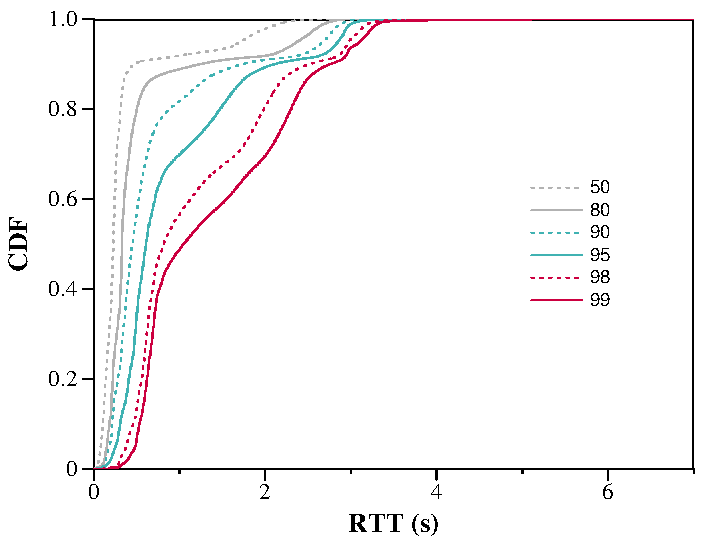
\includegraphics[width=0.7\textwidth]{timeouts/figs/cdf_raw_ping_ttl}
\end{center}
\caption{\label{fig:raw_lat}%
CDF of percentile latency of survey-detected responses per IP address: Each point represents an IP address
and each curve represents the percentile from that IP address's
response latencies. The slope of the latency
percentiles increases around the 3 second mark, suggesting that
ISI's prober timed out responses that arrived after 3 seconds.
}
\end{figure}

In this section, we present the latencies we would observe
when considering only those responses that were matched to 
requests because they arrived within the timeout.  We call 
these responses \emph{survey-detected responses}.

We aggregate round trip time measurements in terms of the
distribution of latency values per IP address, focusing on
characteristic values on the median, 80th, 90th, 95th, 98th
and 99th percentile latencies.  That is, we attempt to treat
each IP address equally, rather than treat each ping
measurement equally.  This aggregation ensures that
well-connected hosts that reply reliably are not
over-represented relative to hosts that reply infrequently.

Taking ISI survey datasets from 2011--2013 together, we show a CDF of
these percentile values considering only survey-detected
responses in Figure~\ref{fig:raw_lat}.  Taken literally, 95\%
of echo replies from 95\% of addresses will arrive in less than
2.85 seconds.  However, it is apparent that the distribution
is clipped at the 3 second mark, although a few responses
were matched even after 7 seconds.   

We observe three broad phases in this graph: (1) the lower
40\% of addresses show a reasonably tight distribution in
which the 99th percentile stays close to the 98th; (2) the
next 50\% in which the median remains low but the higher
percentiles increase; and (3) the top 10\% where the median
rises above 0.5 seconds.


\subsection{Unmatched responses}

If a probe takes more than three seconds to solicit a
response, it appears as if the probe timed-out and the
response was unsolicited or \emph{unmatched}.  Since it
appears from Figure~\ref{fig:raw_lat} that three seconds is
short enough that it is altering the distribution of round
trip times, we are interested in matching these echo
responses to construct the complete distribution of round
trip times.

Matching these responses to find \emph{delayed responses} is
not a simple matter, however.  In particular, we find two
causes of \emph{unexpected responses} that should not yield
samples of round trip times: unmatched responses solicited
by echo requests sent to broadcast addresses and apparent
denial of service responses.

% We require the union of low-rtt responses' latencies and high-rtt
% responses' latencies to perform an analysis of ping
% latencies. 
% \subsection{Matching delayed responses}

We match a delayed response with its corresponding request
as follows: Given an unmatched response having a source IP
address, we look for the last request sent to that IP
address.  If the last request timed out and has not been matched, the latency is then the difference between the
timestamp of the response and the timestamp of the
request.  ISI recorded the timestamp of unmatched responses
to a 1 second precision, thus the latencies of inferred
delayed responses are precise only to a second.

The presence of unexpected responses can lead to the
inference of incorrect latencies for delayed responses using
this technique: not all unexpected responses should be
matched by source address.
We thus develop filters to remove unexpected responses from the set of
unmatched responses.

We note that it is possible to match responses to requests
explicitly using the id and sequence numbers associated with
ICMP echo requests, and even perhaps using the payload.
These attributes were not recorded in the ISI dataset, which
motivates us to develop the source address based scheme.  We
use these fields when running Zmap or other tools to confirm
high latencies in Section~\ref{sec:verification} below.


% Some of
% these unmatched responses are higher latency responses which arrived
% at the prober after the timeout duration; we call these responses high-rtt
% responses. The remaining unmatched responses are unexpected responses, sent either
% in response to an echo request addressed to a broadcast address or as part
% of a Denial of Service attack. 

% \subsection{Unexpected Responses}
% 
% The dataset contains two sources of unexpected responses: Responses
% obtained from probes sent to broadcast addresses and
% duplicate responses.  We discuss each in turn. 
% Our goal is to study the latency of pings, including both low-rtt as
% well as high-rtt responses. To recover high-rtt responses from the
% data, we need to match unmatched echo Responses with their corresponding echo Requests.

% Have a figure here which shows the distribution of latencies from the
% raw pings, and how we found out that it has a 3 second timeout.
% ISI has a timeout of 3 seconds. Drop everything that arrives after
% then.

% When we tried reconstructing, we had to clean up a bunch. Had the
% following problems:

\subsubsection{Broadcast responses}

% We show that several unmatched responses are caused by
The dataset contains several instances where a ping to a
destination times out, but is closely followed by an
unmatched response from a source address that is within the same /24
address block, but different from the destination.
% The dataset contains several unmatched
% responses that were received immediately after a ping was sent to a different
% address within the same /24 address block.
In each round of probing, this behavior repeats.
%
Here, we analyze these unmatched responses, find that they are likely
caused by probing broadcast addresses, and filter them.

Network prefixes often include a broadcast address, where one
address within a subnet represents all devices connected to
that prefix~\cite{rfc919}.
%
The broadcast address in a network should
be an address that is
unlikely to be assigned to a real host~\cite{rfc919}, such as the
address whose host-part bits are all 1s or 0s, allowing us to
characterize broadcast addresses.
%
Devices that receive an echo
request sent to the broadcast address may, depending on
configuration, send a response~\cite{rfc1122}, and if sending a response,
will use a source address that is their own.
%
We call these
responses \emph{broadcast responses}.  
%
No device should send
an echo response with the source address that is the
broadcast destination of the echo request. 

% We investigate Echo Requests to destination addresses that trigger
% Echo Response from different addresses within the same /24 address blocks.
% We seek to understand why an Echo Request sent to a destination
% address would trigger an Echo Response from a different address within
% the same /24 address block.
% We hypothesize that a ping sent to broadcast address triggers
% responses from address(es) within the same /24 address block.
We hypothesize that pings that trigger responses from different
addresses within the same /24 address block result when the
ping destination is a broadcast address. 
We examine ping destinations
that solicit a response from a different address in the same /24
address block, and check if they appear to be broadcast addresses.
%
%
% These addresses will have last octets that
% can be represented as $2^n-1$ such as 63, 127, 255 etc.
%
% We wondered if network operators are following this convention.
%

We extended the ICMP probing module in the
Zmap scanner~\cite{durumeric2013zmap} to embed the destination
into the echo request, then to extract the destination from the
echo response.
%
Doing so allows us to infer the destination address to which the probe
was originally sent.
%
% We mark such a response as a
% broadcast response.
%
Zmap collected the data and made
it available for download at \url{scans.io}.
%

We choose the Zmap scan conducted closest in
time to the last ISI survey we studied, on April 17 2015, to investigate
the host-part bits of destination addresses that triggered responses
from a different address from the same /24 address block.
%
We plot the distribution of the last octets of these addresses in
Figure~\ref{fig:zmap_last_octet_hist}.
%
Last octets with the last N bits ending in 1 or 0, where N is greater than 1,
such as 255, 0, 127, 128 etc., have spikes. These addresses are likely broadcast addresses.
% Last octets with the last N bits as 1 (where N $>$ 1), such as 255, 127, etc., have the largest
% spikes. Last octets with the last N bits as 0, such as 0, 128, etc.,
% also have spikes, but smaller.
On the other hand, last octets that
end in binary '01' or '10' have very few addresses.

\begin{figure}[t]
\begin{center}
\includegraphics[width=3in]{timeouts/figs/zmap_last_octet_hist_all_bcast_addrs_apr_17}
\end{center}
\caption{\label{fig:zmap_last_octet_hist}%
Broadcast addresses that solicit responses in Zmap: Broadcast addresses usually
have last octets whose last N bits are either 1 or 0
(where N $>$ 1).
}
\end{figure}


\subsubsection*{Broadcast responses exist in the dataset}

% Next, we show the existence of broadcast responses in the ISI dataset.
% We examine how many of the unmatched responses in the dataset are
% broadcast responses. 
%
\begin{figure}[t]
\begin{center}
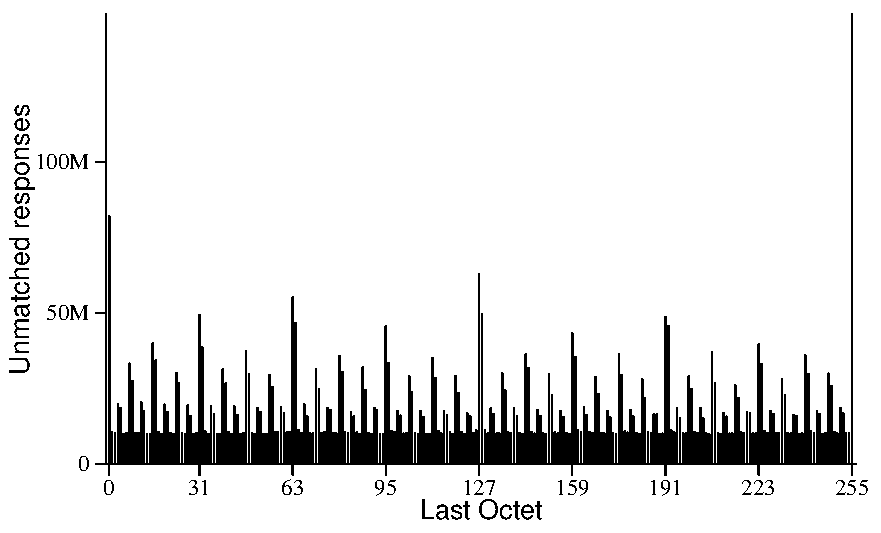
\includegraphics[width=.99\linewidth]{timeouts/figs/last_octet_hist}
\end{center}
\caption{\label{fig:bcast_hist}%
Number of unmatched responses that followed a probe sent to address
with last octet X. Last octets with last N bits ending in
0s and 1s (where N $>$ 1) observe spikes, likely caused by broadcast
responses. Not all unmatched responses are caused by broadcast
responses, however, since there exist roughly 10M unmatched
responses distributed evenly across all last octets.}
\end{figure}



We examine if unmatched responses in the ISI dataset are caused by pings sent to broadcast addresses.
%
Since broadcast responses are likely to be seen after an
Echo Request sent to a broadcast address, we find
the most recently probed address within the same /24 prefix for each
unmatched response. 
%
We then extract the last octet of the most recently probed
address.
%
Figure~\ref{fig:bcast_hist} shows the
distribution of unmatched responses across these last octets. 
%
We find that around 10M unmatched responses are distributed evenly
across all last octets: these are unmatched responses that don't seem
to be broadcast responses.
%
However, last octets that have their last N bits as 1s and 0s
,when N is greater than 1, observe spikes similar to those in Figure~\ref{fig:zmap_last_octet_hist}.
% , supporting our hypothesis that these are
% responses to broadcast addresses.
%
% These are the addresses most likely to see an
% unmatched response after an echo request to them times
% out. 
%

If left in the data, broadcast responses could yield
substantial latency overestimates in the following, common,
scenario, which we illustrate in
Figure~\ref{fig:bcast_sample}.
%
Assume that the echo request
sent to an address 211.4.10.254 is lost and that the
device is configured to respond to broadcast pings.  
%
The
echo request sent to 211.4.10.254 could then be matched to
the response to the request sent to 211.4.10.255, the
broadcast address of the enclosing prefix.  
%
This would lead
to a latency based on the interval between probing
211.4.10.254 and 211.4.10.255, as shown in the figure.

\begin{figure}[t]
\begin{center}
% \centering
% 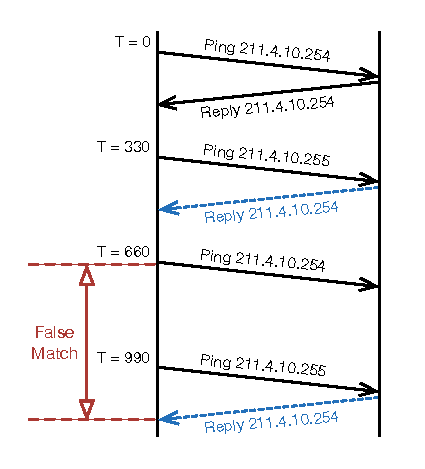
\includegraphics[width=0.97\linewidth]{timeouts/figs/wfall_bcast}
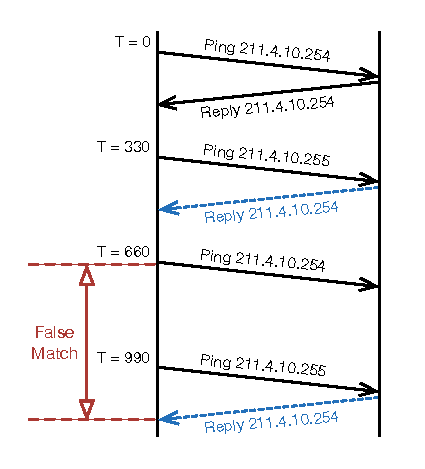
\includegraphics[width=3in]{timeouts/figs/wfall_bcast}
\end{center}
\caption{\label{fig:bcast_sample}%
We filter broadcast responses since they can lead to the inference of
false latencies. This figure illustrates a potential incorrect match
caused by a broadcast response.
Echo requests sent to the broadcast address 211.4.10.255 at T = 330
and T = 990 seconds solicit responses from 211.4.10.254.  When a timeout occurs 
for a request sent directly to 211.4.10.254 at T = 660 seconds, we 
would falsely connect that request to the response at T = 990 seconds.}
\end{figure}

%
% A last octet of 255 and 0 have particularly large spikes, 
% corresponding to the possible broadcast addresses of a /24 subnet.

\subsubsection*{Filtering broadcast responses}

% A potential approach to filtering broadcast responses is to check
% if an unmatched response was preceded by a ping to an address
% whose last octet had its last N bits as 1s or 0s (where N $>$ 1).
% %
% However, this scheme would have been too aggressive, potentially filtering
% delayed responses that coincidentally happened to arrive after an Echo
% Request to a broadcast address.
% %
% Thus, we develop an alternate method which uses ISI's non-random probing
% scheme to detect addresses that source broadcast responses.
%
We develop a method which uses ISI's non-random probing
scheme to detect addresses that source broadcast responses.
We call such addresses \emph{broadcast responders}, and seek to filter
all their responses.
 % and the assumption that broadcast responses, like typical Echo
% responses, have stable latencies.
%
We believe that delayed responses are likely to
exhibit high variance in their response latencies, since congestion varies over
time. 
%
On the other hand, a
broadcast response is likely to have relatively stable latency.
%
% (unless it happens to be congested too.)

ISI's probing scheme sends
probes to each address in a /24 address block in a nonrandom sequence,
allowing us to develop a filter that checks if a source address responds
to a broadcast address each round.
%
% The last octet of the probed IP address generally has its $n$th
% bit (counting from 0) swapped every $2^n$ probes on the /24 block.
Addresses are probed such that last octets that are off by one, such
as 254 and 255, receive pings spaced 330 seconds apart (half the
probing interval of 11 minutes) as shown in Figure~\ref{fig:bcast_sample}.
% nth most significant bit probed, i.e., probes to 1 and 129 are sent
% one after the other.
%
% We filter broadcast responses by looking for unmatched responses from
% the same source address that
% repeat periodically with similar latency.
%
For every unmatched response with a latency of at least 10 seconds,
the filter checks if the same source address had sent an unmatched
response with a similar latency in the previous round.
% checks whether they occurred right before another response of a
% similar latency (within 2 seconds).
%
We take an exponentially weighted moving average of the number of times
this occurs for a given source address with $\alpha=0.01$.
%
Most broadcast responders have the
maximum of this moving average $>$ 0.9, but since probe-loss can
potentially decrease this value, we mark IP addresses with values $>$
0.2 and filter all their responses. 
%
% If the maximum of this moving average per source address is greater than 0.2, the IP address
% is marked as one that responds to probes to broadcast addresses, and
% it is filtered out.
% %
% This filter is meant to be selective for the specific pattern of responses, without being so
% selective that it fails to classify broadcast addresses in the
% presence of loss.

We confirm that we find broadcast responders correctly in the
ISI surveys by comparing the ones we found in the ISI 2015 surveys
with broadcast responders from the Zmap dataset.
%
% Ideally, the Zmap scan should have been conducted at the same time as
% the ISI surveys, but we choose the closest available Zmap scan in time,
% bearing in mind that broadcast responders may change over time.
%
% The IT63w (20150117)
% and IT63c (20150206) datasets recorded responses from 4,008,830
% addresses.
% %
% The filter detected 9,942 broadcast responders among them.
%
% 8729 of these broadcast responders appeared as the source addresses
% of an Echo Response in Zmap's
% April 17 2015 scan. 
%
Zmap detected 939,559 broadcast responders in the April 17
2015 scan, of which 7212 had been
addresses that provided Echo Responses in ISI's IT63w (20150117) and
IT63c (20150206) datasets.
%
The filter detected 7044 (97.7\%) of these as broadcast responders. 
% We inspected the remaining 168 addresses and found that 159 could not have been broadcast responders at the time they were probed by ISI: their 99th percentile RTTs were far too low.
We inspected the 168 remaining addresses and found that 154 addresses
have 99th percentile latencies below 2.5 seconds. Since ISI
probes a /24 prefix only once every 2.5 seconds, these addresses
cannot be broadcast responders. Another 5 addresses have 99th
percentiles latencies below 5 seconds; these are unlikely to be
broadcast responders as well.

The remaining 9 addresses had 99th percentile latencies in excess of
300s and seem to be broadcast responders. Upon closer inspection, we
found that these addresses only occasionally sent an unmatched
response: around once every 50 rounds. The $\alpha$ parameter of the
filter can tolerate some rounds with missing responses, but these
addresses respond in so few rounds that they pass undetected. 
If these 9 are indeed broadcast responders as suggested by high 99th percentile latencies, this yields a false negative rate of our filter of 0.13\%.
% demonstrating that it is able to find broadcast responders with high
% accuracy.

\subsubsection{Duplicate responses}

Packets can be duplicated.  A duplicated packet will not affect inferred latencies as
long as the original response to the original probe packet reaches the prober, since our scheme
ignores subsequent duplicate responses. However, we find that some IP
addresses respond many times to a single probe. In this case, the incoming packets aren't responses to
probes, but are either caused by incorrect configurations or malicious
behavior. 

\begin{figure}[t]
\begin{center}
% \centering
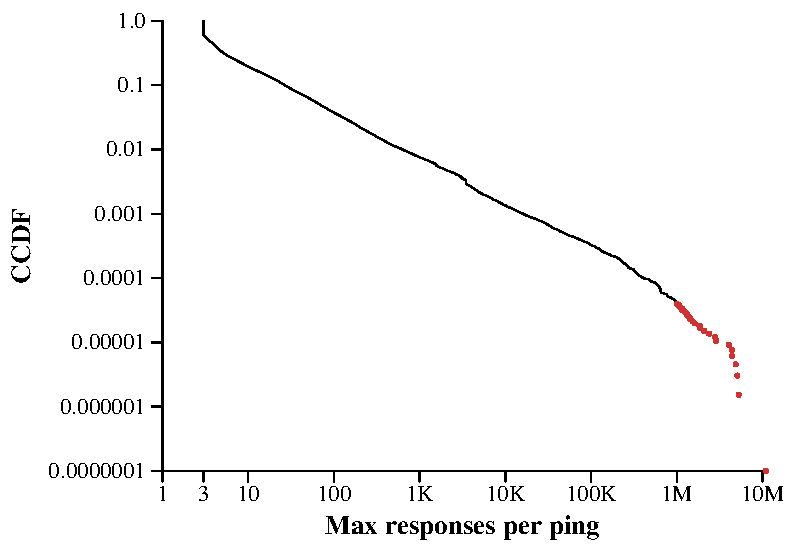
\includegraphics[width=.9\linewidth]{timeouts/figs/ccdf_dos}
\end{center}
\caption{\label{fig:dos}%
Maximum number of responses received for a single echo request, for IP
addresses that sent more than 2 responses to an echo request. The red
dots indicate instances where addresses responded to a single echo
request with more than 1M echo responses. We believe that these are
caused by DoS attacks.}
\end{figure}

Figure~\ref{fig:dos} shows the distribution of the maximum number of
echo responses observed in response to a single echo request. Since
broadcast responses can also be interpreted as duplicate responses, we
look only at IP addresses that sent more than 2 echo responses for an
echo request. Of 658,841 such addresses, we find that 4,985 (0.7\%) sent
at least 1,000 echo responses. The red dots in the figure show 26
addresses that sent more than one million echo
responses, with one address sending nearly 11 million responses in 11 minutes.

Zmap authors reported that they observed
retaliatory DoS attacks
in response to their Internet-wide probes~\cite{durumeric2013zmap}. We believe that
some of the responses in the ISI dataset are also caused by DoS attacks.

We filter duplicate responses by ignoring IP addresses that ever
responded more than 4 times to a single echo request, based on observing the
distribution of duplicates shown in Figure~\ref{fig:dos}.  Packets can
sometimes get duplicated on the Internet, and we want to be selective
in our filtering to remove as little as necessary.  Even if a response from
the probed IP address is duplicated and a broadcast response is also
duplicated, there should be only 4 echo responses in the dataset. We
believe that IP addresses observing more than 4 echo responses to a
single echo request are either misconfigured or are participating in a DoS attack.
In either case, the latencies are not trustworthy.


% \vfill\eject
\section{Recommended Timeout Values}
\label{sec:eval}
% \newcommand{\hdr}[1]{\multicolumn{1}{c}{\textbf{#1}}}

In this section, we analyze the ping latencies of all pings obtained
from ISI's Internet survey datasets from 2015 to find reasonable timeout values.
We demonstrate the effectiveness
of our matching scheme for recovering delayed responses from the
dataset. We then group the survey-detected responses and delayed
responses together to determine what timeout values would be necessary to 
recover various percentiles of responses. 
Some IP
addresses observe very high latencies in the ISI dataset; we verify that
these are real in Section~\ref{sec:verification} and examine causes in Section~\ref{sec:causes}.

% we validate
% our results by probing these IP addresses with the scamper tool~\cite{luckie2010scamper} and
% analyzing their latencies.

\subsection{Incorporating unmatched responses}

\begin{table}[tb]
  \begin{center}
    \begin{small}
  \begin{tabular}{c|rr}
    & \hdr{Packets} & \hdr{Addresses} \\
    \hline
    \textbf{Survey-detected } & 9,644,670,150 & 4,008,703\Tstrut\\
    % \hline
    \textbf{Naive matching} & 9,768,703,324 & 4,008,830 \\
    % \hline
    \textbf{Broadcast responses} & 33,775,148 & 9,942 \\
    % \hline
    \textbf{Duplicate responses} & 67,183,853 & 20,736 \\
    % \hline
    % \textbf{Filtered survey-detected} & 125,578,194,082 & 16,320,357 \\
    % \hline
    \textbf{Survey + Delayed} & 9,667,744,323 & 3,978,152 \\
    \end{tabular}
    \end{small}
  \end{center}
    \caption[Adding unmatched responses to survey-detected responses]{
\label{tbl:filter_results}
Adding unmatched responses to survey-detected responses}
\end{table}

\begin{figure*}[tb]
\begin{subfigure}[t]{0.47\linewidth}
\centering
\includegraphics[width=\linewidth]{timeouts/figs/cdf_basic_ping_ttl}
\caption{
\label{fig:basic_lat}
Before filtering
}
\end{subfigure}
%
\hfill
%
\begin{subfigure}[t]{0.47\linewidth}
\centering
\includegraphics[width=\linewidth]{timeouts/figs/cdf_filter_ping_ttl}
\caption{
\label{fig:filter_lat}
After filtering
}
\end{subfigure}
\caption{
\label{fig:lat} 
CDF of Percentile latency per IP address before and after filtering
  unexpected responses. Each point represents an IP address and each
  color represents the percentile from that IP address's response
  latencies. Before filtering unexpected responses, there are
  bumps caused by broadcast responses at 330s, 165s and 495s,
  fractions of the 11 minute (660s) probing interval.
}
\end{figure*}


ISI detected 9.64 Billion echo responses from 4 Million IP addresses in 2015
in the IT63w (20150117) and IT63c (20150206) datasets, as shown in the
first row of Table~\ref{tbl:filter_results}.
The next row shows the number of responses we would have obtained
if we had used a naive matching scheme where we simply matched each
unmatched response for an IP address with the last echo request for
that IP
address, without filtering unexpected responses.
The number of responses
increases by 1.3\% to 9.77 Billion; however, this includes responses
from addresses that received broadcast responses and duplicate
responses. 
%
After filtering unexpected responses, the number of IP addresses
reduces to 99.23\% of
the original addresses. 
%
Of 30,678 discarded IP addresses, 9,942 (32.4\%)
addresses were discarded because they also received broadcast
responses. 
%
The majority of discarded IP addresses, 20,736 (67.6\%) were addresses that
sent more than 4 echo responses in response to a single echo request. 

Though the number of discarded IP addresses is relatively small, removing
them eliminates responses that cluster around 330, 165, and 495 seconds.
Figure~\ref{fig:lat} shows the distribution of percentile latency per
IP address before and after filtering unexpected responses.  Comparing
these two graphs shows that the ``bumps'' in the CDF are removed by the filtering.

After discarding addresses, our matching technique yields 23,074,173
additional responses for the remaining addresses, giving us a total of
9.67 Billion Echo Responses from 3.98 Million IP addresses. We perform
our latency analysis on this combined dataset.

% They are caused
% because of the non-random sequence of probing, which meant that 0 and
% 1 were probed 330seconds apart.

% \newcommand{\bb}{~~~~~}
%%% \begin{table}[tp]%
%%%   \begin{center}%
%%%   \begin{small}%
%%%   \begin{tabular}{c@{\hspace{0.5em}}r|rrrrrrr}
%%%     &\multicolumn{8}{c}{\textbf{\% of pings}\vspace{0.3em}} \\
%%%     && \hdr{1\%} & \multicolumn{1}{c}{\textbf{50\%}} & \hdr{80\%} & \hdr{90\%} & \hdr{95\%} &
%%%     \hdr{98\%} & \hdr{99\%} \\\cline{2-9}
%%%     \parbox[t]{2mm}{\multirow{7}{*}{\rotatebox[origin=c]{90}{\textbf{\% of addresses}}}} & 
%%%     \textbf{1\%} & 0.01 & 0.05 & 0.11 & 0.13 & 0.16 & 0.29 & 0.34 \\
%%% %    \cline{2-9}
%%%     &\textbf{50\%} & 0.12 & 0.24 & 0.35 & 0.50 & 0.67 & 0.92 & 1.21 \\
%%% %    \cline{2-9}
%%%     &\textbf{80\%} & 0.19 & 0.33 & 0.57 & 1.34 & 2.20 & 5\bb & 7\bb \\
%%% %    \cline{2-9}
%%%     &\textbf{90\%} & 0.24 & 1.00 & 2.39 & 4\bb & 6\bb & 8\bb & 11\bb \\
%%% %    \cline{2-9}
%%%     &\textbf{95\%} & 0.31 & 2.43 & 5\bb & 6\bb & 7\bb & 12\bb & 18\bb \\
%%% %    \cline{2-9}
%%%     &\textbf{98\%} & 0.37 & 4\bb & 6\bb & 7\bb & 11\bb & 20\bb & 52\bb \\
%%% %    \cline{2-9}
%%%     &\textbf{99\%} & 0.43 & 4\bb & 6\bb & 8\bb & 14\bb & 55\bb & 159\bb \\
%%%     \end{tabular}
%%%   \end{small}
%%%   \end{center}
%%% 
%%% 
%%%     \caption{Minimum timeout in seconds that would have captured c\% of pings from r\% of IP
%%%       addresses in pings sent from Nov 2011 to October 2013 (where r is the row number and c is
%%%       the column number).}
%%% \label{tbl:grand}
%%% \end{table}

%\newcommand{\bb}{~~~~~}


\subsection{Recommended Timeout Values}

We now find retransmission thresholds which recover various
percentiles of responses for the IP addresses from the
combined dataset. For each IP address, we find the 1st, 50th, 80th,
90th, 95th, 98th and 99th percentile latencies. We then find the 1st, 50th,
80th, 90th, 95th, 98th and 99th percentiles of all the 1st percentile latencies. We repeat this for each
percentile and show the results in Table~\ref{tbl:grand_2015}.

\begin{table}[tb]
  % \begin{center}%
    \begin{small}%
      \hspace{-0.06in}%
  \begin{tabular}{l@{\hspace{0.5em}}r|rrrrrrr}
    &\multicolumn{8}{c}{\textbf{\% of pings}} \\
    && \hdr{1\%} & \multicolumn{1}{c}{\textbf{50\%}} & \hdr{80\%} & \hdr{90\%} & \hdr{95\%} &
    \hdr{98\%} & \hdr{99\%} \\\cline{2-9}
    \multirow{7}{*}{\rotatebox[origin=lb]{90}{\textbf{\% of addresses}}} & 
    \textbf{1\%} & 0.01 & 0.03 & 0.04 & 0.07 & 0.10 & 0.13 & 0.18\Tstrut \\
%    \cline{2-9}
    &\textbf{50\%} & 0.16 & 0.19 & 0.21 & 0.26 & 0.42 & 0.53 & 0.64 \\
%    \cline{2-9}
    &\textbf{80\%} & 0.19 & 0.26 & 0.33 & 0.43 & 0.54 & 0.74 & 1.21 \\
%    \cline{2-9}
    &\textbf{90\%} & 0.22 & 0.31 & 0.42 & 0.57 & 0.84 & 1.61 & 3\bb \\
%    \cline{2-9}
    &\textbf{95\%} & 0.25 & 1.42 & 2.38 & 3\bb & 5\bb & 9\bb & 15\bb \\
%    \cline{2-9}
    &\textbf{98\%} & 0.30 & 1.94 & 4\bb & 6\bb & 12\bb & 41\bb & 78\bb \\
%    \cline{2-9}
    &\textbf{99\%} & 0.33 & 2.31 & 4\bb & 8\bb & 22\bb & 76\bb & 145\bb \\
    \end{tabular}
    \end{small}
    % \end{center}

\vspace{\baselineskip}
    \caption[Minimum timeouts]{Minimum timeout in seconds that would have captured c\% of pings from r\% of IP
      addresses in the IT63w (20150117) and IT63c (20150206) datasets (where r is the row number and c is
      the column number).}
\label{tbl:grand_2015}
\end{table}

The 1st percentile of an address's latency will be close to the ideal latency that its link
can provide. We find that the 1st percentile latency is below 330ms for 99\%
of IP addresses: most addresses are capable of
responding with low latency. Further, 50\% of pings from 50\% of the
addresses have latencies below 190ms, showing that latencies tend to
be low in general.

However, we see that a substantial fraction of IP addresses also have
surprisingly high latencies. For instance, to capture 95\% of pings from 95\%
addresses requires waiting 5 seconds.  Restated, at least 5\% of
pings from 5\% of addresses have latencies higher than 5 seconds. Thus, even
setting a timeout as high as 5 seconds will infer a false loss rate of 5\%
for these addresses.

Note that retrying lost pings cannot be used as a substitute for
setting a longer timeout since a retried ping is not an independent
sample of latency. 
Whatever caused the first one to be delayed is likely to cause the
followup pings to be delayed as well, as we show in Section~\ref{sec:causes}.

At the extreme, we see 1\% of pings from 1\% of addresses
having latency above 145 seconds! These latencies are so high that
we investigate these addresses further.  \emph{We now
  consider 60 seconds to be a reasonable timeout to balance
  progress with response rate, at least when studying
  outages and latencies, although an ideal timeout may vary
  for different settings.}  A timeout of 60 seconds easily
covers 98\% of pings to 98\% of addresses, yet does not seem
long enough to slow measurements unnecessarily.


\section{Verification of long ping times}
\label{sec:verification}

In this section, we address doubts that long observed ping
times are real: that they are a product of ISI's probing scheme, that
they might be caused by errors in a particular data set, or that they might derive from
discrimination against ICMP.

\subsection{Are high latencies observed by other probing schemes?}

Some of the latencies in Table~\ref{tbl:grand_2015} are so high that
we considered if they could be artifacts of ISI's probing scheme. We
investigate latencies obtained using two other probing techniques,
Zmap and scamper, and check if the high latencies observed in the ISI datasets are reproducible.
%  We confirm that each observes the
% occurrence of long ping times.
% We use the scamper tool to probe a subset of high
% latency addresses and 



\subsubsection*{Does Zmap observe high latencies?}
% \paragraph{Zmap observes high latencies}

We check for high latencies using the Zmap scanner~\cite{durumeric2013zmap}. 
%
As part of our extension of the ICMP probing module in the
Zmap scanner, we also embed the probe send time into the echo request,
and extract it from the
echo response, allowing us to estimate the RTT, albeit without the
precision of kernel send timestamps.
%
% Zmap collected the data and made
% it available for download at \url{scans.io}.

Zmap has performed these scans since April 2015. Scans have been conducted over a range of different times,
different days of the week and across four months in 2015 (as of Sep
5, 2015), as shown in Table~\ref{tbl:scans}. Typically, scans were performed on Sundays or Thursdays, beginning
at noon UTC time. However, the scans on April 17, May 22, and June 15
were conducted on other days and at other times, increasing diversity. Each Zmap scan
takes 10 and a half hours to complete and recovers Echo Responses from
around 350M addresses.
%

\begin{table}[tb]
  \begin{center}
    \begin{tiny}
  \begin{tabular}{r|c|c|c}
    \hdr{Scan Date} & \hdr{Day} & \hdr{Begin Time} & \hdr{Echo Responses} \\
    \hline
    \textbf{Apr 17, 2015} & Fri & 02:44 & 339M\Tstrut \\
    \textbf{Apr 19, 2015} & Sun & 12:07 & 340M \\
    \textbf{Apr 23, 2015} & Thu & 12:07 & 343M \\
    \textbf{Apr 26, 2015} & Sun & 12:07 & 343M \\
    \textbf{Apr 30, 2015} & Thu & 12:08 &  344M \\
    \textbf{May 3, 2015} & Sun & 12:08 & 344M \\
    \textbf{May 17, 2015} & Sun & 12:09 &  347M \\
    \textbf{May 22, 2015} & Fri & 00:57 & 371M \\
    \textbf{May 24, 2015} & Sun & 12:09 &  369M \\
    \textbf{May 31, 2015} & Sun & 12:09 & 362M \\
    \textbf{Jun 4, 2015} & Thu & 12:10 & 368M \\
    \textbf{Jun 15, 2015} & Mon & 13:53 & 357M \\
    % \hline
    \textbf{Jun 21, 2015} & Sun & 12:11 & 368M \\
    % \hline
    \textbf{Jul 2, 2015} & Thu & 12:00 & 369M \\
    \textbf{Jul 5, 2015} & Sun & 12:00 & 368M \\
    \textbf{Jul 9, 2015} & Thu & 12:00 & 369M \\
    \textbf{Jul 12, 2015} & Sun & 12:00 & 367M \\
    \end{tabular}
    \end{tiny}
  \end{center}
    \caption[Details of Zmap scans used in the analyses]{Zmap scan details: For each Zmap scan in
      Figure~\ref{fig:grand_zmap}, the table shows the date, day of the
      week, the time at which the scan began (in UTC time), and the number of
      destinations that responded with Echo Responses.}

\label{tbl:scans}
\end{table}

We choose all
available scans and 
analyze the distribution of
RTTs for the Echo Responses in
Figure~\ref{fig:grand_zmap}. 
%
Most responses arrive with low latency, having a median latency lower than
250ms for each scan.
%
However, ~5\% of addresses responded with RTTs greater than 1 second
in each scan. Further, 0.1\% of addresses responded with latencies exceeding
75 seconds in each scan although the 99.9th percentile
latency exhibited some variation: the May 22 scan had the lowest 99.9th percentile
latency (77 seconds) whereas the July 9 scan had the highest (102 seconds).
%
We infer from these nearly identical latency distributions that high latencies are persistent for a consistent fraction of addresses.
% To compare the distribution of RTTs requires choosing a
% comparable sample from the survey data, given that it
% reprobes addresses for weeks.  We used the latency of the
% first received ping from each address in the IT63c
% (20150206) and IT63w (20150117) datasets.  

% Figure~\ref{fig:zmap_vs_isi_2015} shows the distribution of RTTs. 5\%
% of addresses have latencies $>$ 1s in each.

% \begin{figure}[tbh]
% \centering
% \includegraphics[width=3in]{figs/zmap_vs_isi_2015}
% \caption{\label{fig:zmap_vs_isi_2015}%
% Distribution of RTTs for three Zmap scans and
% two ISI surveys performed in 2015. 5\% of addresses have latencies $>$
% 1s in each.
% }
% \end{figure}

\begin{figure}[tb]
% \centering
\begin{center}
\includegraphics[width=3in]{timeouts/figs/grand_zmap}
\end{center}
\caption[Distribution of RTTs for all Zmap scans performed in 2015]{\label{fig:grand_zmap}%
Distribution of RTTs for all Zmap scans performed in 2015. Around 5\%
of addresses have latencies greater than 1s in each scan, and 0.1\% of addresses observed latencies in excess of 75s.
}
\end{figure}

% \vspace{-0.1in}

\subsubsection*{Does scamper also observe high latencies?}
% \paragraph{Scamper also observes high latencies}
Both ISI and Zmap probe millions of addresses, and we investigate
whether latencies are affected by these probing schemes
triggering rate-limits or firewalls. We select a small sample of
addresses that are likely to have high latencies from the
ISI dataset, probe them using scamper~\cite{luckie2010scamper}, and check for unusually high latencies.

In the 2011 - 2013
ISI dataset, 20,095 IP
addresses had at least 5\% of their pings with latencies 100 seconds and above. We chose 2000 random IP addresses from
this subset and sent 1000 pings to them, once every 10 seconds using
scamper~\cite{luckie2010scamper} and analyzed the responses. 
In this
analysis, we used scamper's default packet response matching
mechanism: so long as scamper continues to run, received responses
will be matched with sent packets. Because we used scamper's defaults,
scamper ceased to run 2 seconds after the last packet was sent, so
we missed responses to the last few pings that arrived after
scamper ceased running. Although scamper can
be configured to wait longer for responses, in later analyses, we ran tcpdump simultaneously and matched
responses to sent packets separately.

Of the 2000 addresses, 1244 responded to our probes.
Figure~\ref{fig:cdf_high_rtt_ips} shows the percentile latency per IP
address. The 95th percentile latency for 50\% of the addresses is now
considerably lower, at 7.3s. This suggests that addresses prone to extremely high
latencies vary with time: we investigate addresses with
this behavior further in Section~\ref{sec:causes}. 

Nevertheless, Figure~\ref{fig:cdf_high_rtt_ips} shows that scamper
also observes some instances of very high latencies. 17\%
of addresses observe latencies greater than 100 seconds for 1\%
of their pings. We therefore rule out the possibility that the high
latencies are a product of the probing scheme.

% , and show that they addresses tend
% to be from cellular Autonomous Systems which exhib


\begin{figure}[tb]
\begin{center}
% \centering
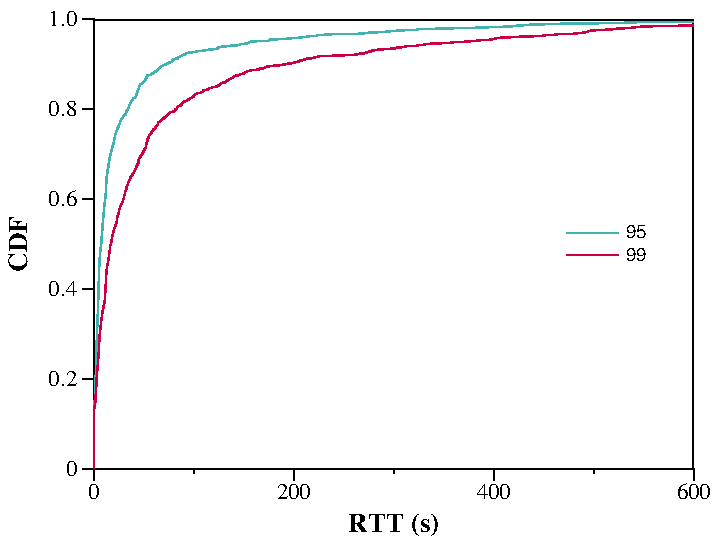
\includegraphics[width=3in]{timeouts/figs/cdf_high_rtt_guys_grand}
\end{center}
\caption[Confirmation of high latency with Scamper]{\label{fig:cdf_high_rtt_ips}%
Confirmation of high latency: Percentile latency per IP address for
2000 randomly chosen IP addresses from ISI's 2011 - 2013 surveys that had $>$ 5\% of pings with
latencies 100s and above. Each point represents an IP address and the
lines represent the percentile latency from that IP address. 17\% of
them continue to observe 1\% of their pings with
latencies $>$ 100s.
}
\end{figure}

% \subsection{Are ISI's sampled addresses representative?}

% ISI's methodology involves probing a sample of the address
% space.  It would be reasonable to expect that perhaps this
% sampling affects observed latencies.  An underestimate might
% occur because a fraction of the ISI survey prefixes have
% been repeated since 2006, so such addresses may be in a more
% established part of the network.  On the other hand,
% latencies might be overestimated by bad luck, repeatedly probing a
% particularly slow prefix. 


% 0.1% of pings arrived after: April : 90, May : 77,  June : 83, Julys
% : 102

% per dataset analysis (time)
\ninput{timeouts/per_dataset}

\ninput{timeouts/is_it_icmp}

\subsection{Summary}

In this section, we confirmed that extremely high latencies are also observed by
techniques besides ISI's. We find that the high latencies are
not a result of a few individual ISI datasets, even though some
did appear atypical.  Further, high latencies affect all
protocols the same. 

We also found that the prevalence of high latencies has been increasing
since 2011. In 2015, a consistent 5\% of addresses have
latencies greater than a second. 

%% 
%% * could it be routing? (if affecting all of a /24 at the same time;  I don't believe this happens)
%% 
%% * could it be handoff?  (should be occasional / rare (though not necessarily so), within some networks but not all, and apply to networks with already high latencies)
%% 
%% * could it be solar interference on satellites?  (seek diurnal patterns s.t. for one (15 minute?) period out of the 24 hours, there's a problem)
%% 
%% * does it affect thought-to-be-wired links?  (seek large cable-provider networks and fiber providers, determine whether there are high latency guys in there.)
%% 
%% * can the devices be fingerprinted? (e.g., nmap)

\section{Why do pings take so long?}
\label{sec:causes}

In this section, we aim to determine what causes high RTTs. We
investigate the RTTs of satellite
links and find that they account for a small fraction of high RTT
addresses. We follow up with an analysis of Autonomous Systems and
geographic locations that are most prone to two potentially different
types of high RTTs: RTTs greater than 1s and RTTs greater than
100s. We then investigate addresses that exhibit each type of RTT and
find potential explanations.
% check if the first ping to an address in a continuous stream of pings is subject to
% higher latencies than the rest. Finally, we investigate particularly high
% latencies and identify patterns associated with their occurrence.

\ninput{timeouts/satellites}

\ninput{timeouts/zmap_asn_analysis}

\ninput{timeouts/first_ping}

\ninput{timeouts/handoff}

\subsection{Summary}
High latencies appear to be a property mainly of cellular
  Autonomous Systems, though a few also appear on satellite
  links. Latencies in the ISI data that are regularly above one second seem to be caused
by the first-ping behavior associated with several addresses, where
the first ping in a stream of pings has higher latency than the
rest. Egregiously high latencies, i.e., latencies greater than a
hundred seconds, occur in two broad patterns. In the first, latencies
steadily decay with each probe, as if clearing a backlog. In the second, latencies are continuously
high and are accompanied by loss, as if the network link is oversubscribed.



\section{Conclusion and Discussion}

Researchers use tools like ping to detect network outages,
but generally guessed at the timeout after which a ping
should be declared ``failed'' and an outage suspected.  The
choice of timeout can affect the accuracy and timeliness of
outage detection: if too small, the outage detector may
falsely assert an outage in the presence of congestion; if
too large, the outage detector may not pass the outage along
quickly for confirmation or diagnosis.

We investigated the latencies of responses in the ISI survey
dataset to determine a good timeout, considering the
distributions of latencies on a per-destination basis.
Foremost, latencies are higher than we expected, based on
conventional wisdom, and appear to have been increasing.
We show that these high latencies are not an artifact of
measurement choices such as using ICMP or the particular
vantage points or probing schemes used, although different data sets vary somewhat.
We show that high latencies are not caused by links with a substantial
base timeout, such as satellite links.  
% 
% 
% We analyzed the latencies of echo responses, including
% unmatched responses in the ISI survey data set, to determine
% what timeout would capture different fractions of
% responses from different fractions of remote IP addresses.
% We showed that high latencies are not an artifact of ISI
% data. % , and in fact, it may underestimate the extent of large latencies by sampling.
% We showed that high latencies are not an artifact of using ICMP
% echo requests: prioritization that might favor data-carrying TCP or UDP
% protocols does not have this substantial of an effect.
% We showed that high latencies have been increasing over the
% last few years by comparing different surveys taken at different times.
% We showed that satellite links are not particularly blameworthy
% in requiring high timeout values.
Finally, we showed that in many instances, the initial communication to
cellular wireless devices is largely to blame for high latency measures.
Similar spikes that may be consistent with handoff also dissipate over time,
to more conventional latencies that support application traffic.
With this data, researchers should be able to reason about
what to expect in terms of false outage detection for a
given timeout and how to design probing methods to account for
these behaviors.

% Our initial hypothesis was that it would be a simple matter
% to confirm that widely used timeout values would be adequate
% for studying outages, or failing that, that one or two
% additional seconds would be enough.
As memory capacity and performance becomes less of a
limiting factor, we believe that the lesson of this work is
to design network measurement software to approach outage
detection using a method comparable to that of TCP: send
another probe after 3 seconds, but continue listening for a
response to earlier probes, at least for a duration based, at
least in part, on the error rates implied by
Table~\ref{tbl:grand_2015}. 
% We plan
% to use 60 seconds when we need a timeout, and avoid timeouts
% otherwise.

% a per-ISP
% and per-region basis, since there can be wide variation in
% latencies. This work provides timeout values that would capture most
% pings (say 99\%) per-ISP and per-region. 

% The wide variation in observed latencies for IP addresses around the
% world indicate that probers should set timeout values
% based upon the addresses that they are probing. Even a 3s
% timeout may suffice for 90\% of addresses in the ISI survey since 90\% of addresses respond
% within 3s for 99\% of the pings sent to them. 

If investigating historical outage measurement data collected by
probing based techniques, the timeouts used by the technique must be
compared with timeouts that would have captured almost all responses
for the addresses pinged by the technique. For example, Thunderping
probes addresses only in the U.S. For these addresses, both the ISI
and Zmap datasets showed that more than 99\% of ping responses arrived
within the 5s timeout used by Thunderping. The probability of false
outage inferences due to high latency is small. However, if the Thunderping
technique had been used to ping addresses in South American cellular
ISPs, there would be a significantly higher probability of detecting
false outages, since the 5s timeout would have missed many delayed responses.

% In cases where a timeout is 


% My proposed work is to find expected latency values
% associated with the IP addresses that need to be probed, and to set
% their timeouts accordingly.
 
% I propose to find expected latencies for any IP address on the
% Internet by analyzing historical and current ping data, available from
% the Zmap project~\cite{censys-icmp}. Zmap has continued to perform
% their scans of the IPv4 Internet, averaging one scan per week since
% April 2015. For each IP address that has consistently responded to
% pings, I expect to have roughly 100 samples. I will calculate expected
% latencies for all addresses using their own latencies weighted by the
% number of observed samples and will also include latency samples of
% other ``related'' addresses. Related addresses can be addresses
% belonging to the same /24 network, addresses belonging to the same
% ISP, addresses sharing the same last-hop router, addresses from the
% same dynamically addressed pools etc; I describe related addresses in
% more detail in Section~\ref{sec:last_mile}.

% Once I have determined the expected latencies for all IP addresses
% that respond to pings in the IPv4 Internet, the next task is to
% determine appropriate per-address timeouts based upon the destinations
% that need to be probed. Given any address to probe, I will modify the probing scheme to
% set timeouts that are just high enough as to capture almost all
% responses (say 99.9\%) from that address. Setting adaptive timeouts this way will achieve the
% twin goals of capturing most responses while also keeping the state
% required at the prober low.


\chapter{Mitigating false inferences due to dynamic addressing}

\label{cpt:addr_change}

% TODO: Index section numbers to the roadmap

In this chapter, I begin by describing a common assumption---that IP
addresses can be used as proxies---for users in
Section~\ref{sec:addrs-are-host-proxies}. In
Section~\ref{sec:addrchange-false-inferences}, I discuss how dynamic
addressing can lead probing-based outage detection techniques to make
false inferences about outages.

Next, I describe work with colleagues to empirically
measure the frequency of dynamic addressing and the durations for
which addresses are assigned to residential home router devices in
several networks around the world and the effect of outages upon
dynamic reassignment~\cite{addrchange-reasons}. The measurements we
used are sourced from the RIPE NCC's Atlas project, which deploys small devices, called probes, that
conduct measurements from globally distributed
networks~\cite{atlas}. The RIPE Atlas dataset offers measurements that allow us to
determine when an IP address change occurred and what the addresses
were before and after the change. In addition, the dataset includes many
measurements that provide context about what was happening around the
time of the address change. I was able to use these measurements to
detect when RIPE Atlas probes rebooted and were not sending pings
(indicating a power outage) and when their pings were not getting
responses (indicating a network outage). In a study with colleagues of active RIPE
Atlas probes in 2015, we found 3,038 RIPE Atlas probes with address
changes hosted across 929 ISPs and 156
countries~\cite{addrchange-reasons}. Using the measurements from RIPE Atlas, I identify networks
where addresses are typically stable. 

Finally, in section~\ref{sec:complementary-ns} I discuss a technique to identify outages even in networks
where dynamic reassignment is common. Using a complementary dataset
that allows checking if an address for which a probing-based technique
detected an outage has remained the same before and after the detected
outage, we are able to confirm outages even in networks where dynamic
reassignment is common.

\section{IP addresses can be proxies for end users}

\label{sec:addrs-are-host-proxies}

Academia and industry often rely on a simplifying assumption that IP
addresses uniquely identify
end-hosts~\cite{p2pfilesharing,p2pavail,sen2004analyzing,sekar2006multi,anomalousdns,kuhrer2015going,xie2005worm,jung2004empirical,fabian2007botnet,stone2009your,andriesse2015reliable,fail2ban,spamhaus,cbl,sorbs}. This
assumption allows researchers to track end host behavior over
time~\cite{anomalousdns, kuhrer2015going, pingin}, or to count
participating users in peer-to-peer
systems~\cite{p2pfilesharing,p2pavail,sen2004analyzing}. Many
organizations create blacklists of suspicious IP addresses based on
previously observed malicious traffic associated with those
addresses~\cite{fail2ban,spamhaus,cbl,sorbs}. 

Probing-based techniques like Thunderping~\cite{pingin} make a similar
assumption: a probed address is representative of a residential
customer's Internet connection. Many residences have at least one
device with a public IP address~\cite{cgn-imc16}, typically the home
router. When a home router's address stops responding
to pings, it could be evidence of a residential Internet outage.

All of these applications would benefit from understanding how often
and when dynamic addresses assigned to user devices change.

\section{Probing-based techniques can make false outage inferences due
to dynamic addressing}

\label{sec:addrchange-false-inferences}

When probing-based remote outage detection techniques send probes to an address, they expect that the
address continues to be assigned to the same end-host for the entirety
of the probing duration. Depending upon how a dynamic address gets
reassigned, these techniques can make false inferences about outages in two ways:

\begin{itemize}

\item{\emph{Detecting false outages} Probing-based remote outage detection techniques detect outages
    when a previously responsive address stops responding to
    probes. However, If a dynamic address being probed is
withdrawn from its host and is not assigned to any other host, active probes to the address will no longer
elicit responses. These techniques will infer false
probe-loss, leading them to infer false outages.}

\item{\emph{Detecting false outage duration} These techniques detect outage
    duration by continuing to probe an unresponsive address. When the
    address starts responding to probes again, the outage is inferred
    to end. If a home router with a
    public dynamic address has an outage and at some point during the outage,
    the dynamic address is reassigned to some other home router
    which responds to probes, probing-based remote outage detection techniques would infer that the outage ended incorrectly.
% For ISPs that use DHCP
%     for address assignment, we would expect dynamically
%     assigned addresses to stick around on the end-host until an
%     outage occurs. However, upon the occurrence of the outage, if the
%     outage is long enough, they can get reassigned to another host,
%     especially, if the outage is longer than the DHCP lease
%     duration. Here, RODWAP techniques can detect the outage itself but
%     can perhaps not detect outages that are long
}

% TODO: CITE http://www.umiacs.umd.edu/~tdumitra/courses/ENEE757/Fall15/papers/Stone-Gross09.pdf
\end{itemize}

My approach to mitigating these false inferences is to analyze how
frequently and for what reasons dynamic addresses are reassigned, in
various networks. Using the results of these analysis, I identify
networks where addresses are typically stable. 

% TODO: Think about whether I want the following text in the diss.

% I will use the results of these analyses to build a model
% of how likely an inference about an outage using a probing-based
% remote outage detection technique is
% a false inference caused by dynamic addressing. For example,
% preliminary work with colleagues has revealed that some European ISPs change addresses upon
% very small outages and are particularly likely to change addresses at certain
% times of the day~\cite{addrchange-reasons}. These results will inform
% my model to not attempt detection of 
% outage duration for these ISPs, and to discard outages
% detected at times that are particularly likely to have dynamic address
% changes. The model will ultimately yield stable addresses who either
% do not undergo dynamic reassignment for months at a time, or who get
% reassigned but in a predictable manner. Thunderping limits itself to
% probing addresses in the U.S. where dynamic reassignment is
% uncommon~\cite{addrchange-reasons}; stable addresses from the
% model can help us detect outages in new areas.




% The results from the dynamic DNS dataset are preliminary in
% scale and based on a short measurement to show potential.
% Further, our study of RIPE Atlas data showed us that the cause of
% address changes is important. I intend to couple our
% outage-detection tool to probe addresses corresponding to
% the dynamic DNS domains while fetching their A records.  We
% can thus identify outages that occur near the reassignment,
% allowing us to infer if an address-change was caused by an outage and
% feed results into the model. Further, if the dynamic DNS result
% indicates that a probed address had recently been reassigned, then the
% detected false positive outage can be filtered.
 
% \subsubsection{Open DNS resolvers}

% Since 2010, various studies have reported on the existence of more
% than 15 million 'open' DNS resolvers on the
% Internet~\cite{openresolver, schomp2014clientsidedns, kuhrer2014exit,
%   kuhrer2015going}. These DNS resolvers are 'open' because they will resolve a DNS query sent from arbitrary IP
% addresses on the Internet. Previous studies have found that more than
% three-quarters of open DNS resolvers are likely to be
% residential~\cite{schomp2014dnsvul, schomp2014clientsidedns}. I
% propose two potential approaches to fingerprint these open DNS
% resolvers and track address changes.

% \paragraph{DNS caches}
% Open DNS resolvers often cache previous
% lookups~\cite{schomp2014dnsvul}. My insight is that these caches can
% be used to fingerprint open DNS resolvers, allowing us to track when
% their IP addresses change. I plan to do this in two phases.

% First, I will find open DNS resolvers on the Internet. I propose to register a domain and deploy an Authoritative DNS server
% for it. Then I intend to perform a one-time scan of the entire IPv4
% address space by sending a DNS request for a subdomain within the
% domain we control to all the IPv4 addresses on the Internet. Each DNS
% request I send to a target IP address will embed the target address
% into the request, similar to the approach used by Dagon et
% al.~\cite{dagon2008corrupted}. The Open DNS resolvers will route the
% request to our Authoritative DNS server.  At the authoritative DNS
% server, I will note the target IP address to which this request was
% sent and generate a unique fingerprint for the device at this address,
% and embed this fingerprint in my response. When these responses
% reach the open DNS resolvers, each will now contain its unique
% fingerprint in its cache.

% Next, I will periodically inspect the caches of known open DNS resolvers.
% I will issue periodic DNS requests for the subdomain we
% control (with the target IP address embedded in the request) to all
% the addresses that contacted our Authoritative DNS server. If we
% obtain the fingerprint that we had previously issued to that address,
% we know that the device continues to be assigned that address. If we
% find that an address is no longer returning the expected cache
% fingerprint, we know that the address has changed. I then propose to
% issue DNS requests to related addresses (as described in
% Section~\ref{sec:last_mile}) with the \emph{old} target IP address
% embedded in the request. If the device is present on any of those
% addresses, then we will obtain the expected fingerprint. Upon finding
% the device at a new address, we will update
% our local mapping and note that the fingerprint is now available at
% this new address.

% \paragraph{Anomalous Open DNS Resolvers}

% Of the 30 million Open DNS Resolvers on the Internet, around 17
% million are \emph{anomalous}~\cite{anomalousdns}, i.e.,
% instead of sending DNS responses with a source port of 53, they
% respond with a non-standard source port. Kaizer et al. ~\cite{anomalousdns} found that
% these devices are primarily residential ADSL modems. Not only do these
% devices use a non-standard source port, DNS requests can be made to
% these devices in such a way that the source ports are assigned
% \emph{sequentially}. My insight is that we can use this sequential
% assignment of source ports to fingerprint anomalous open DNS resolvers.

% The first part of our approach here is similar to my approach with
% the DNS caches: I will find open DNS resolvers that are anomalous. After registering a domain and deploying an Authoritative DNS server
% for it, I will perform a one-time scan of the entire IPv4
% address space by sending a DNS request for a subdomain within the
% domain we control to all the IPv4 addresses on the Internet. Each DNS
% request I send to a target IP address will embed the target address
% into the request as before. However, instead of embedding responses with
% unique fingerprints from the authoritative DNS server, we simply
% monitor the source ports that issue DNS responses from each
% address. If it's a non-standard port, we flag the device as an
% anomalous open DNS resolver.

% Next, I will periodically inspect the source ports used by anomalous
% open DNS resolver responses. Since we know which
%   addresses the anomalous open DNS resolvers are located at, I
%   periodically issue DNS queries to these addresses. As long as the
%   source port for successive requests to an address continues to be
%   sequential, I can state with high confidence that the address has
%   not changed. The source ports for these devices typically vary
%   between 10,000 to 30,000; thus there is only a small likelihood that
%   another device coincidentally happens to have the next value in
%   sequence. If we find that a response doesn't arrive, or that one
%   arrives but the source port is not sequential, then we know that the
%   device's address has been reassigned. As in the DNS cache approach,
%   I will then look for the expected source port in DNS responses from
%   requests sent to related addresses to find the device again.


% \subsection{Confirming that detected outages are accurate}

% After mitigating false positive outages, I propose the use of datasets
% from RIPE Atlas probes~\cite{atlas} as ground truth to confirm that the remaining
% outages are indeed true positives. In previous work, I had inferred outages occurring on
% RIPE Atlas probes by looking for gaps when probes did not perform 
% measurements that they were scheduled to~\cite{addrchange-reasons}. By
% probing IP addresses at which RIPE Atlas probes are also deployed, I
% will compare outages we detect against outages inferred from RIPE
% Atlas datasets and validate whether our detected outages are accurate.

\label{cpt:weather}

% \chapter{Analyzing the effect of external factors upon Internet
%   reliability}
\chapter{Analyzing weather's effect on Internet Reliability}
\label{cpt:weather}

One aspect of measuring Internet reliability is to determine if the occurrence of certain events adversely affects Internet connectivity. Consider the occurrence of adverse weather conditions for instance: prior work has shown that Internet outages occur more frequently during times of precipitation~\cite{pingin}. However, this work was preliminary in nature and was performed over a short duration (three months). Further, it treated every instance of a previously responsive address failing to respond to pings as an outage, ignoring the effects of dynamic addressing.

In this section, I discuss a technique to quantify the effect of
external factors, such as the occurrence of various weather
conditions, upon Internet connectivity of residential addresses using
measurements from the Thunderping probing system~\cite{pingin}. The
technique mitigates false outages due to dynamic addressing and user
behavior. First, I verify that weather conditions do not positively
correlate with peak diurnal failure periods, where dynamic addressing
or false outages due to user behavior are common. Next, I quantify
the absolute increase in the number of outages observed during
weather, when compared to non-weather periods---the outage
inflation---for several types of weather including times with
precipitation and times with extreme temperatures and high winds. By
studying outage inflation of various link types and geographic regions
across weather conditions, I am able to identify networks that are
vulnerable to weather.

\subsection{Thunderping measurement system}

Thunderping probes addresses during times of severe weather. 

\subsection{Find the inflation in dropout rate}

The key insight here is that determining the inflation in \emph{dropout} rate when event(s) occur captures the increased likelihood of the \emph{outage} rate. 

% \begin{figure*}[t]
% %
% \begin{subfigure}[t]{0.47\linewidth}
% \centering
% \includegraphics[width=\linewidth]{figs/frate_by_timeofweek_jan11todec17_scatter}
% \caption{
% \label{fig:frate_lts_timeofweek}
% Dropout probability has significant diurnal variation.
% }
% \end{subfigure}
% %
% \hfill
% %
% \begin{subfigure}[t]{0.47\linewidth}
% \centering
% \includegraphics[width=\linewidth]{figs/addresshoursbywtyp_by_timeofweek_scatter}
% \caption{
% \label{fig:weather_timeofweek}
% Different weather conditions are prominent at different times.
% }
% \end{subfigure}
% %
% \caption{
%  Weather does not occur most often during hours of the week when there are an inflated number of dropouts. 
% }
% \end{figure*}



 
\section{Introduction}

Wather-related damage to vital infrastructure
(in this case the power grid) can lead to significant economic harm.
%
Yet, %  in the Internet era,
little is known about the economic impact of
weather-induced outages on the most pervasive infrastructure that people use to
access the Internet: residential last-mile links.
%
For massive last-mile outages, telcos are required by U.S.~policy~\cite{cfr49}
to report the outage to the FCC.
%
However, the minimum reporting threshold is astronomical: the outage must be at
least 30 minutes in duration, and it must have affected tens of thousands of
customers~\cite{cfr49}.
%
Researchers have also studied widespread link failures in the Internet,
like undersea cable cuts~\cite{chan-pam11, bilski-ccis09}, natural
disasters~\cite{heidemann-sandy}, and backbone router
failures~\cite{iannaccone-imw02}. 

In practice, most weather events are much more localized and not severe enough
to generate such a large outage.
%
For decades, this everyday weather has been known to lead to to smaller scale
outages of telecom infrastructure.
%
For example, early telephone and cable television engineering documents
describe how to avoid moisture in wires because it impedes signal
propagation~\cite{aiee09-jewett, toct66-smith}.  Also, rain attenuates
satellite signals above 10~GHz~\cite{ieee75-hogg}.  Finally, point-to-point
wireless links can experience multipath fading due to objects moving in the
wind~\cite{ieeecm01-bolcskei}. In short, residential links are vulnerable to
everyday weather because residential equipment and wiring are often installed
outdoors: wind can blow trees onto overhead wires, heat can cause equipment to
fail, and rain can seep into underground equipment cabinets.
 
Surprisingly, for these everyday weather conditions, there are no public
statistics on the frequency or magnitude of the outages they induce (directly
and indirectly).
%
This could be a problem for Internet-based companies because they do not know
how many customers they are losing to nature, and for regulators because they
do not know how significant the problem is, and which conditions and geographic
areas deserve their attention.
%
In this work we resolve this issue: we provide the first comprehensive study
that identifies the correlation between everyday weather and residential
Internet last-mile outages.
%
Specifically, we quantify the absolute increase in the number of outages
observed during weather, when compared to non-weather periods.

%To make this information useful to the intended audience of this work (i.e.,
%policymakers, web companies, and operators), 

Quantifying the relationship between occurrences of weather and an increase in
outages cannot be answered with a short term %, broadly collected
study.
%
The data set needs to be longitudinal because weather is
\emph{seasonal}---certain weather conditions only happen at certain times of
year---and because some weather events are \emph{rare} enough that providers in a 
specific location may not be adequately prepared.
%
Targeted probing is needed because weather is \emph{localized}: at any time
only specific geographic locations are exposed to weather conditions.
%
Broad observation of outages of several links will capture correlated outages
of several hosts, such as the work by Heidemann et al.~\cite{imc08-heidemann,
trinocular}, but it will not reveal failures of individual links as may be
the case for weather.
%
Although some systems can obtain detailed measurements at residential
gateways~\cite{ripe-atlas,sundaresan-sigcomm11}, the limited deployment of
these measurement systems make them inadequate for studying the scale needed to
observe many different weather conditions, multiple times, in different
geographic areas.
%
Therefore, we performed a seven year longitudinal study with targeted
measurements of residential links surviving weather events.

In 2011, we introduced a measurement system for this task called
ThunderPing~\cite{schulman-imc11}.
%
For the past seven years ThunderPing has been following forecasts of weather in
the U.S. and pinging a sample of 100 hosts from each last-mile provider in the
area for six hours before, during, and six hours after the forecasted weather
event.
%
The focus of our initial paper on ThunderPing was its probing methodology, but
it also included a preliminary study that looked at 66 days of data.
%
Given how limited the data set was, we were unable to draw statistically 
significant conclusions and we saw only one season, summer, of one
year. % ---therefore we could not, with any confidence, quantify the increase in
% outages during weather events.
%
We also did not have enough data to explore variations in effect of
weather by geography,
%
nor could we explore if the likelihood of failure varies
with continuous weather conditions (e.g., wind speed),
 
In this paper, the time totaled across all responsive links
exposed to different weather events is in the \textbf{centuries}.
%
For example,
we have observed a total of \emph{100 centuries} of DSL links exposed to cold
weather.
%
This large data set enabled us to address all of these significant limitations
of our prior preliminary study.
 
There is a challenge with quantifying how weather correlates with
outages: outages are relatively uncommon events, and thus every outage
is a significant event.
%
%This means every single outage is a significant event.
%
This is compounded by the fact that we wish to analyze subsets of our
data to focus on, say, particular link types or locations.
%% Yet, we need to slice and dice the data to isolate different properties
%% of residential links that may be related to their failure likelihood:
%% namely their link type and location.
%
With so few outages observed compared to the time that links are responsive,
it is difficult to determine if different weather causes a statistically significant
increase in outages.
%
To address this issue, we borrow statistical tools from epidemiology
that enable us to reason about the \emph{inflation} in dropout
probability, and to establish statistical significance to our results,
even though failures happen at relatively low rates.
%
We detail this approach in Section~\ref{sec:hazard}, as we believe it
to be of general use to the community.


%% known as
%% \emph{hazard rate}.
%% %
%% This tool enables us to establish statistical significance of our results, even
%% though there are relatively few failure events.
%% %
%% This metric enables us to measure the \emph{increase} in probability of a failure
%% that correlates with a specific type, or intensity, of weather.
%% 
%% We expect that this metric may be useful for web and cloud service operators
%% because they can use it to quantify how many of the outages that they observe
%% are likely due to weather alone, and thus estimate how much revenue they are
%% losing to weather outages.
%% %
%% It may be useful for regulators because they can determine if the added number of
%% failures from weather is significant enough to warrant new policy focused on
%% addressing weather outages, such as advocating for undergrounding
%% infrastructure as it has a demonstrated improvement on robustness to
%% weather~\cite{undergrounding}.

Another challenge is this metric could be artificially inflated by
weather conditions coinciding with daily network state changes such as
maintenance or renumbering~\cite{addrchange-imc}.
%
We verify that weather does not appear to be positively correlated with
peak diurnal failure periods, and to do recovery time analysis we
select networks and outage durations unlikely to suffer from address
renumbering, allowing us to ensure that we are probing the same
residential link before and after the outage.

\paragraph{Observations and Contributions}
%
We present a dataset spanning seven years, all weather conditions, and
76~billion responsive pings to 8.7~million hosts throughout the U.S. 
%
We apply techniques from epidemiology to attribute statistically
significant rates of dropout to individual weather conditions.
%
Our key findings span four broad areas of analysis:

\begin{itemize}

\item \textbf{Link type variations} (\S\ref{sec:inflations}): Different link
types experience weather in highly varying ways.  For instance, compared to
wired link types (cable, DSL, fiber), wireless link types (WISPs and satellite)
experience greater increases in dropout rates during rainy conditions and high
temperatures, but often \emph{decreases} in dropout rates in snow and cold
temperatures.

\item \textbf{Geographic variations} (\S\ref{sec:geography}): Different
geographic regions can be affected to varying degrees.  For instance,
Midwestern U.S.~states are more prone to failures in thunderstorms and rain
than coastal states.  Southern states are more prone to failures in snow than
other states.

\item \textbf{Continuous variable analysis} (\S\ref{sec:continuous}): Most link
types have highly nonlinear dropout rates with respect to changes in
temperature, wind speed, and precipitation.  For temperature, dropout rates are
typically non-monotonic; satellite links drop out more in moderate temperatures
than low or high temperatures.

% \item \textbf{Recovery times} (\S\ref{sec:recovery}): The amount of time to
% recover from a dropout varies significantly across different weather
% conditions.  Thunderstorms take the longest for cable links to recover from.

\end{itemize}

Our findings have ramifications on how network outage detection and analysis
should be performed; limiting measurements to any particular geographic region,
link type, or time of year can introduce statistically significant bias.
%
We believe our results also have implications for network administrators and
policy-makers; an increased use of satellite links in the Midwestern U.S.~has
resulted in those states' increased dropout rates in rainy weather.
%
We will be making all of our data and code publicly available.

% New contributions =============================================================

% Can quantify weather because we have more data

% Tons more data allowed us to compute confidence intervals

% Double checking if we have more failures due to maintenance periods and what not

% Failure duration 

% Double checking if failure duration with NetSession data

% Each of the PLOTS, DUH!

% Extra text {{{

% Among our findings, we show that temperature has a
% surprising relationship with link reliability: extreme
% temperature correlates with failures of typical link types,
% while satellite links and dialup links see high failure at
% modest temperatures.  Wind degrades reliability proportional
% to the square of wind speed, and the amount of hourly
% precipitation, in contrast, has a less pronounced effect on
% reliability.  However, the type of precipitation has a
% substantial effect---freezing rain, hail, and thunderstorm
% often double the probability of seeing a failure, depending 
% on link type.

% 
% A location can be exposed to the same weather patterns year over year, then one
% year a severe storm such as Hurricane Sandy in New York City in 2012.
% %
% This is important for our study because it will reveal how resilient last-mile
% Internet links are to failures when an anomalous weather event occurs that
% providers are not prepared for.
% 
% Therefore, the seven years worth of data that we collected for this study
% provides an opportunity to quantify the effect of weather on a particular
% location.
%

% Unlike the measurements needed to understand
% these failures, the collecting measurements needed to understand residential link failures
% requires a particularly broad set of hosts. Weather 
% varies by location and time, and how residential hosts fail in weather 
% depends on location, link type, and Internet service provider.

% Evaluation of weather-related failures in this work presented in
% Section~\ref{sec:failurerate} are backed with more pings which enable
% statistical comparisons between failures in different weather conditions, and
% observations of continuous weather conditions such as wind speed and
% temperature.

% For the continuous weather measurements, we observe clear
% relationships between the probability of failure depending on the residential
% link type~\todo{nums}. For the discrete weather measurements, we observe~\todo{nums}.

% With both breadth and depth, the observations of residential link
% failures can also be correlated with other possible causes: We study weather as
% a likely cause of outages to gain confidence that outages can be detected
% remotely; this confidence enables future comparisons of reliability measures
% across providers and countries.


% Weather can cause fixed \lastmile transmission media to
% fail~\cite{schulman-imc11}. 
% 
% Also there are so many different ISPs that it is difficult to get a global
% picture of the weather-related failures.
% 
% We know a lot about how loss of vital infrastructure affects business from the supplier side.
% %
% We do not however know what the costs are of having customers disconnected due to weather.
% In this work we deliver on that promise
% 
% 
% Unlike other vital infrastructure, residential Internet depends on the operation
% of other vital infrastructure to function.
% %
% Also, it has a lower barrier for a user to shut it down on their own, in
% particular to avoid damage of their equipment during storms.
% %
% If it does turn out that users are doing this, this is still valuable knowledge
% for operators as those customers will not be able to access their networks.
% 
% 
% (1) Categorical
%  - overall
%  - geographic (rama finds the worst link type/geography combination)
%}}}


\section{Data Set}

This section describes the data we collected and its initial
processing.
%
We start with a definition of the partially interpreted data
we seek: ``dropouts,'' where an address fails to respond in
the context of otherwise ``responsive hours'' of an address.
%
Dropouts and \emph{disruptions} from Chapter~\ref{cpt:corrfails} are synonymous.
%
We next briefly review the ThunderPing data probing system and
present brief statistics about the raw active probing data.
% 
Then, we review the weather data, particularly how and
where it is collected and how we handle hurricanes.
%
We conclude by describing the benefits (and limitations) of this
data for our study of weather-related effects.

\subsection{Dropouts, Defined} %{{{

A dropout happens when the address attached to a residential link transitions from
being responsive to pings from multiple vantage points, to being unresponsive
from all of the vantage points.
% 
Specifically, we define a residential link ``dropout'' as an hour when at least three
vantage points pinging a host and receiving replies suddenly experience 11 minutes
(an entire probing interval) where they do not receive a 
reply before a five second timeout.
%
This dropout occurs within a ``responsive address hour,'' a
continuous observation of an IP address in known weather
conditions.  A responsive hour may or may not include a
dropout, and the ratio of dropouts to responsive hours is a
measure of outage likelihood.  Responsive hours add: two
addresses both observed in the same hour or one address
observed for two hours in the same conditions are equivalent.

Our selection of three vantage points is based on prior work's selection
of three vantage points to observe outages~\cite{trinocular}.
%
Our selection of a five second timeout for ping responses is based on our
prior work that observed that most ping replies to residential
hosts are received within five seconds~\cite{timeouts}.
%
Our selection of one hour as the time period for a dropout is based on the fact
that the weather data we collected consists of hourly reports.
%
Considering at most one dropout per probed address per hour will diminish the
number of observed dropouts from individual links, if they should alternate
between responsive and unresponsive states: there can be at most one per hour,
not five (due to the 11 minute probing interval).

% To contrast with a dropout, a ``responsive hour'' is an hour
% in which weather is experienced, but the address does not
% experience a dropout.
% We define responsive hour later in Sec 2.4. And we do it
%   correctly there!
% nspring - I think it needs to be here, corrected if necessary.

Observing a dropout is a sign that a residential link may (but may not) have
experienced an outage:
%
\emph{Dropouts are a superset of outages.}
%
Dropouts can also occur if the device re-attaches to the
network with a new address after only momentary
disconnection, typically through re-association of a PPP
session for a DSL modem, but potentially through
administrative renumbering of prefixes. For our purposes, we
expect these events to occur independent of weather, such
that the two events can be studied separately.
%
% Restated, when a residential link experiences a prolonged outage, a prolonged
% dropout will also occur.
%
%Other network changes can also lead to dropouts.
%
%IP renumbering is the most common source of dropouts that are not outages. 
%IP renumbering is when residential providers change the IP addresses assigned
%to their customers either via forced renumbering~\cite{forced-renumbering},
%DHCP lease expiration~\cite{dhcp-lease}, or PPPoE sessions
%%expiring~\cite{pppoe}.  For our purposes, we expect these events (address
%reassignment or premise equipment reboot) to occur independent
%of weather, such that the two events can be studied separately.
%
We confirm that dropouts during typical maintenance intervals are
unlikely to correlate with weather in
Section~\ref{subsec:independence_of_maintenance}.
% , and we
% revisit DHCP in Section~\ref{sec:recovery}.

%
% \todo{insert that our approach for dealing with this is statistical?}

In short, by observing dropouts, we will be able to observe how residential
links behave during weather, at the scale necessary to make quantitative
conclusions about weather's effect on residential links in the U.S.
%
% We must also be careful because we observe the effects of
% other network changes that do not correspond with outages.
%}}}

% \subsection{How did we observe if there were dropouts on residential links during weather?} %{{{

\subsection{Dropouts, collected}

We briefly summarize the methodology of ``ThunderPing'': our probing
system that has been running for seven years.
%
More details about ThunderPing can be found in our preliminary work in
%ThunderPing was described in our preliminary work in
IMC~2011~\cite{pingin}.
%, details can be found there.
%
% nspring - I know I wrote this, but I'm not feeling it any more.
% surgical strike preferred.
%Although our initial probing methodology was sufficient for data collection, our
%analysis methods were inadequate in that they did not consider the background
%rate of failures and they were too ambitious in assuming outage duration could
%be understood for all link types.  We describe our revised method in 
%Section~\ref{sec:method}.

The ThunderPing probing methodology is as follows:
%
For every forecast of severe weather provided by the US National Weather
Service, ThunderPing pings a sample of 100 residential hosts from each
provider in the affected region.  The affected region is specified by FIPS code, which roughly
corresponds to counties in the U.S.
%
The probing starts up to six hours before the forecast event, continues during the
event, and terminates six hours after the event, regardless of whether the weather
materializes.
 
The residential hosts ThunderPing pings during each weather event are selected
from a master list of residential hosts classified by provider (reverse DNS
name) and geographic location (FIPS code).  We classify link type by
provider, when the provider implies a well-defined link type; (typically rural) providers that
use a variety of media types to provide connectivity are included under ``All'' link
types with the rest, but are not classified further.  We determine location using a 
MaxMind database from the same year for choosing which addresses to probe, but from the same
month for analysis. Although there are errors in both classifications, a location error
would be expected to cause an underestimate of the effect of weather by placing a host
not in the forecast region falsely into the area of weather effect.
 
ThunderPing sends pings to each of these hosts from up to 10 geographically
dispersed \planetlab vantage points every 11 minutes.  This interval is due to~\cite{imc08-heidemann}.
When a \planetlab node fails, we replace it, but if the number of working vantage points
drops below three, we discard observations at that time as untrustworthy.
%
% Having more than the three vantage points needed to detect dropouts allows us
% to continue probing uninterrupted even in the inevitable case that a
% \planetlab node fails.
% %
When there are at least three, we require
that all active vantage points do not have a response in order to label the event as a dropout.
  
ThunderPing retransmits failed ICMP requests: when a vantage point sees a
lack of ping response it retries that ping with an exponential backoff up to 10
times within the 11~minute probing interval.  Therefore, a dropout will typically require
at least 30 failed ICMP requests.

ThunderPing has been running for seven years, and has
collected 76 billion responsive pings to 8.7 million
residential addresses.
 
\subsection{Weather, classified}

To quantify the effect of weather on dropouts, we needed to determine
what weather residential links were exposed to when a dropout did or did not
occur.

The US National Weather Service (NWS) operates a 
network of 900 automated ``ASOS'' weather stations.
%
These weather stations are typically located at airports.
%
The NWS weather stations record hourly observations of 24 weather
variables in METAR format and make those available~\cite{metar-ftp}.
% nspring: I feel like "we downloaded it" is implied.
%
%For all of the geographic locations that we probed, across all of the time
%periods that we probed, we downloaded METAR data
%from~\cite{metar-ftp}.
%
 
There are two types of weather information: categories that
account for the common precipitation types (e.g.,
thunderstorm, hail, snow) and continuous variables (e.g.,
wind speed, precipitation quantity).

We annotate each responsive address hour for an address with the
corresponding weather information associated with the geographically
closest weather station to that address. Doing so allows us to find
the number of responsive hours and dropout address hours in specific
weather conditions. 

\paragraph{Hurricanes are special}
%
Severe events are among the most important failure events for us to study how the
Internet is affected, as the Internet is increasingly relied on as the primary
mode of communication in an emergency~\cite{emergency-voip-fcc}.
However, severe events have the potential to overwhelm the typical and
obscure interesting observations.

% hurricane_times = [
%    ['October 7 2017 00:00:00', 'October 10 2017 00:00:00'], # Hurricane Nate                  
%    ['September 9 2017 00:00:00', 'September 13 2017 00:00:00'], # Hurricane Irma              
%    ['August 24 2017 00:00:00', 'September 1 2017 00:00:00'], # Hurricane Harvey                
%    ['October 6 2016 00:00:00', 'October 9 2016 00:00:00'], # Hurricane Matthew                
%    ['September 1 2016 00:00:00', 'September 3 2016 00:00:00'], # Hurricane Hermine            
%    ['July 3 2014 00:00:00', 'July 5 2014 00:00:00'], # Hurricane Arthur, don't seem to have an\
% y data                                                                                          
%    ['October 28 2012 00:00:00', 'November 2 2012 00:00:00'], # Hurricane Sandy                
%    ['August 25 2012 00:00:00', 'August 31 2012 00:00:00'], # Hurricane Isaac                  
%    ['August 26 2011 00:00:00', 'August 30 2011 00:00:00'], # Hurricane Irene, don't seem to ha\
% ve any data                                                                                    
% ]

The following hurricanes made US landfall during our
measurement:
Irene (Aug 26--30, 2011),
Isaac (Aug 25--31, 2012),
Sandy (Oct 28--Nov 1, 2012),
Arthur (Jul 3--5, 2014),
Hermine (Sept 1--3, 2016),
Matthew (Oct 6--9, 2016),
Harvey (Oct 6--9, 2017),
Irma (Sept 9--13, 2017), and
Nate (Oct 7--10, 2017)~\cite{noaa-sotc}.
Hurricanes manifest as a combination of weather features and
are so pronounced that their contribution to thunderstorm or
rain outages would be disproportionate.\footnote{It is
  disappointing to realize the irony that the most
  significant weather events are also the least
  surprising.}  We thus omit them from categorical weather
classification (e.g., Figure~\ref{fig:inflatedfrate_by_wtyp_ci_whiskers}).
However, we consider data from Hurricane events
when studying continuous variables (inches of rain and wind speed,
for example, where these extremes are clearly distinguishable).
%
Collectively, these hurricane times account for less than 3\% of
%
%All these hurricane times put together account for less than 3\% of
responsive address hours and 4\% of dropout hours.

\begin{table}
  \hspace{-0.1in}\tiny
\ninput{weather/fragments/summary_table_vert}
  \caption{\label{tbl:summary}Summary of data set for large ISPs
	classified by link type.  ``All'' comprises data from ISPs not
	included in this sample.
	(For this table, we count D.C.~as a state.)
	}
\end{table}



\subsection{Data, Summarized} % Comparing with our IMC 2011 Study}

% \todo{ alter this to cover table 1 and mention the old data in comparison. } 

This data set comprises observations from January 2011 to December 2017,
though only 1467 days included sufficiently many operating vantage points to
classify a responsive address hour.

We show per-ISP highlights in Table~\ref{tbl:summary}.  We
observe major providers such as Comcast, Qwest, and ViaSat
in all fifty states (and DC).  Of the 1.77 Billion
responsive address hours from Table~\ref{tbl:summary}, 139M
(8\%) were hours where responsive addresses experienced
rain, 66M (4\%) snow, and 19M (1\%) thunderstorm.

Contrasted to our preliminary study~\cite{pingin}, this
covers nearly 22 times the duration (compared to 66 days),
and includes roughly 60 times as many dropout events (likely
because those days were in spring and early summer).%
% sentiment in next section :
% is collected over enough time that we can draw
% conclusions with confidence about the increase in dropouts correlated with
% many different types of weather in different geographic locations.
%
\footnote{In the public reviews of the IMC 2011 paper, all of the reviewers stated that
they wished the dataset was more comprehensive so conclusions could be made
about the effects of weather on residential links.}
%
% The dataset in this work covers many seasons several times and contains a 
% severe weather events.
%
%
% At 1467 days, the data in this work spans a period of time 22
% times longer than our preliminary study in 2011.
%

%}}}

\subsection{Why this data?} %{{{

Others have studied outages and collected broad IP
responsiveness data.  Here we describe the benefits
of our data, addressing its limitations in Section~\ref{sec:datasux}.

Our data provides a view on outages of individual addresses,
including isolated outages of ``customer premises''
equipment or singly-connected links that are most exposed.
We rely on statistics to identify a significant change in likelihood of
failure, rather than rely upon large outages of infrastructure
common to a larger aggregate prefix to signify significance.
Every residential link is wired with its
own infrastructure: every residence can have different equipment installed
in different ways and has its own resident network administrator.
As a concrete example, we expect to observe
the effect of water infiltration in the network interface
device (the demarcation point connecting premise phone
wiring to the provider).  (We discuss the flip side of this
coin below.)

Our data is of a scale large enough to compare link
types, providers, geography, and across time.  Seven years
of data make it feasible to observe multiple instances of
both severe and common weather events.  Rare events include
a fair number of tornadoes and virtually unique events such
as snow in Louisiana.  Many observations of similar weather
increase the confidence in our dropout probability estimates,
making it possible to split the data and identify the differences
between, for example, heavy and light rain on wireless ISPs in
Kentucky.  The sampling approach---providing data for each 
provider in an area---ensures that even less-used network links
and providers are well-represented, permitting a comparison with
satellites and wireless ISPs that might be poorly represented
in end host measurement probes~\cite{samknows, sundaresan-sigcomm11,
  ripe-atlas} or when using provider-specific
data~\cite{conext10-jin,cisco-transponder,alpha-transponder}.

Our data includes data from times not subject to interesting
weather: the method probes before and after forecast weather
alerts.  ``Typical'' weather occurs particularly when the
forecast does not materialize or the forecast is for a
long-term event (e.g., summer fire warnings).  With these
measurements, we can establish a baseline for the rate of
dropouts in common weather conditions.  Probing after the
weather also permits measuring recovery time as we wait for
previously responsive addresses to return.

Our data is not sensitive to link failures elsewhere in the
Internet or to PlanetLab vantage point failures.
Restated, with multiple vantage points, catastrophic Internet link outages,
such as the fiber cuts during the ``Baltimore tunnel fire'' in
2001~\cite{bmore-tunnel-fire} will only be considered as an outage if all
vantage points are unable to communicate with the host over the residential
link.  As described above, without three active vantage points,
we make no decision about address responsiveness.

\subsection{Dataset Limitations} % What are the limitations of our data set?} %{{{
\label{sec:datasux}

% \paragraph{Probing is biased to links and time periods where there are weather
% forecasts}
%
The essence of ThunderPing is to selectively probe only when
there is a weather alert forecast for an area, which biases the data
toward time periods where there is some atypical weather present.
Obviously, regions that experience temperate weather are 
unlikely to be represented, and we thus do not attempt to quantify
what fraction of all residential network outages are caused by weather.
More subtly, during the interval around
forecast severe weather, the weather conditions may not be
ideal: our estimate of the background dropout rate is likely inflated 
by proximity to potentially severe weather, thus causing us to underestimate
the quantitative effect of that weather.

% \todo{Aaron- did I capture what you wanted (prior text commented below)?}

% Since ThunderPing only probes when there is a weather forecast for an area, we
% may not probe some residential links that received few or no forecasted weather
% over the course of our seven year study.
% %
% Also, by focusing only on links that are expected to experience weather, we may
% have bias toward hosts that will dropout if our weather assignment is
% incorrect. 
% %
% The result of this is that our baseline number of dropouts may be inflated.

Our approach relies upon active probing to gain breadth
across hundreds of providers, but there are limits to this
breadth: providers may administratively filter ICMP requests
and home routers may decline to respond.  We assume that
providers and end hosts that filter are no more or less
vulnerable to weather and that these features do not affect
our conclusions.

Our data set does not identify the cause of an individual
dropout. Our analysis seeks to correlate observations of
dropouts with weather events under the expectation that a
change in probability of outage is related to the weather.
Should a user turn off equipment nightly, this is
independent of weather and will not not be a factor; should a user
unplug equipment when lightning is nearby, such would
contribute to the probability of dropouts in thunderstorm.
Residential Internet infrastructure is also explicitly reliant
on residential electrical power, and we do not isolate power
failures.  We expect network service outages to be more common
than power outages, for power outages to occur only in the most
severe of weather conditions, and for power outages not
to correlate with link type.
% In part, this is why we omit hurricanes: prior
% studies of network outages in hurricanes were likely to be
% measurements of power loss.~\cite{zmap}

Finally, AT\&T, one of the largest DSL and fiber providers in the US does
not assign reverse DNS names to their residential customers. As such, they
were not included in our master list of residential links that we probe
with ThunderPing.  
%}}}



\chapter{The need for measuring individual address outages}
\label{cpt:corrfails}

In this chapter, I develop and evaluate an approach to detect
dependent \emph{Internet disruption} events that affect multiple residential
addresses simultaneously using measurements of individual address disruptions
gathered with the Thunderping technique. Borrowing terminology from
Richter et al.~\cite{advancing-outage-art}, I define an Internet
disruption event for an address to be the abrupt loss of response to active probing
from that address.

% I define a dependent Internet disruption event to be one which affects
% multiple customers due to a shared underlying cause (such as a network
% or power outage). My insight is that such events can affect multiple
% addresses that are related to each other simultaneously.
Techniques that detect outages at the Internet's edge often seek
disruption events affecting a substantial set of addresses. The set of addresses may comprise
those belonging to the same /24
address block~\cite{trinocular,advancing-outage-art}, BGP
prefix~\cite{hubble}, or country~\cite{dainotti-imc11}.  
Techniques seek such disruption events because individually, each large disruption has
impact and their size makes them easier to confirm, e.g., with operators. In contrast, disruptions
affecting only a few users are harder to detect with confidence.  For example, the
lack of response from a single address might best be explained by a
user switching off their home router---hardly an outage.
However, residential Internet
outages may be limited to a small neighborhood or apartment block; prior
techniques are likely to miss such events.

% In the rest of the chapter, I describe work with colleagues where we
% use a novel approach based upon Binomial hypothesis testing to
% detect instances of per-address disruption events that are unlikely to
% have happened independently and flag these as dependent Internet
% disruption events. Next, we characterize these dependent disruption
% events and present results that challenge conventional wisdom on how
% such disruptions affect Internet address blocks. We show that many of
% these events would be missed by existing techniques that do not
% perform individual address outage detection.

In the rest of this chapter, I describe work with colleagues where we
demonstrate a technique that detects disruption events with
quantifiable confidence, by investigating the potential dependence
between disruptions of multiple IP addresses in a principled way. We
apply a simple statistical method to a large dataset of active probing
measurements towards residential Internet users in the US. We find
times when multiple addresses experience a disruption simultaneously
such that they are unlikely to have occurred independently; we call
the occurrence of such events \emph{dependent disruptions}. We
characterize these dependent disruption events and present results
that challenge conventional wisdom on how such disruptions affect
Internet address blocks. We show that many of these events would be
missed by existing techniques that do not perform individual address
outage detection.

% begin by providing background on why residential
% reliability measurements could require measurements of individual
% addresses' outages. 

\section{Background: dependent residential outages can be small}

Residential Internet connections are vulnerable. The last-mile link
connecting home routers to their ISP is typically not multi-homed and
is therefore a single point of failure. Further, last-mile links can
be damaged by exposure to the elements or by broken tree limbs blown
by the wind. Thus, residential outages may be limited to a small
neighborhood or apartment block.




\section{Conclusion and future work}

In this dissertation, I described how to measure residential Internet
reliability remotely using probing-based techniques. These techni

First, I showed
how to detect Internet outages accurately using these techniques by
analyzing and mitigating potential scenarios that can cause these
techniques to make false inferences about detected outages. 

 can measure Internet
reliability for individual users broadly, longitudinally, and
accurately. In spite of their potential, these techniques can make
false inferences about outages in two scenarios: when probe
responses are delayed beyond timeouts and when addresses get dynamically
reassigned. I described preliminary work which studied how commonly
probes are delayed beyond responses and described measurements of
dynamic addressing across the world that can help build a model of
dynamic addressing. For each outlined scenario, I proposed approaches
that can mitigate false outage inferences when that scenario
occurs. Finally, I discussed an approach to segregate outages into
categories that suggest cause, and how we can use these categorized
outages to study Internet reliability along different dimensions.


\clearpage % TODO: Find out what clearpage does?
\bibliographystyle{plain}
\bibliography{longnames,outages}

\end{document}
